%%%%%%%%%%%%%%%%
% Ph.D. thesis %
%%%%%%%%%%%%%%%%

%\documentclass[11pt,openright,twoside,letterpaper,onecolumn]{report} %% USE THIS FOR DOUBLE SIDED
\documentclass[11pt,openright,oneside,letterpaper,onecolumn]{report}  %% USE THIS FOR SINGLE SIDED

%%%
%%% Packages
%%%
\usepackage[dvips]{epsfig}
\usepackage{amsmath}
\usepackage{named}
\usepackage{fancyhdr}
\usepackage{subcaption}
\usepackage{PMGRefs-defs}

\usepackage{float}


\usepackage[version-1-compatibility]{siunitx}

\usepackage{afterpage}
\usepackage{amsmath}

\newcommand{\thesistitle}{Search for Dark Matter in Proton-Proton Collisions at a Center-of-Mass Energy of 13 TeV in the Higgs Boson associated b-anti-b quark channel}
\newcommand{\thesisauthor}{Jue Chen}
\newcommand{\thesisyear}{2020}

%
% We use the hyperref package and customize it for optimal PDF
%
% Make sure the hyperref is the last package loaded
\usepackage[pdftitle={\thesistitle},pdfauthor={\thesisauthor},pdfpagemode={UseOutlines},letterpaper,bookmarks,bookmarksopen=true,pdfstartview={FitH},bookmarksnumbered=true,colorlinks=true,linkcolor=blue,urlcolor=black,linktoc=all]{hyperref}

%%%
%%% Margins
%%%
\paperwidth=8.5in
\paperheight=11in

% 1in + hoffset + oddsidemargin + textwidth + marginparsep + marginparwidth
% For PhD at Columbia we have single side theses and 1.5in left margin
% The settings below leave 1.5 inch margin at the left and 1 inch at the right
% for US Letter paper
\setlength{\hoffset}{0.0in}
\setlength{\oddsidemargin}{.5in}
\setlength{\textwidth}{6in}
\setlength{\evensidemargin}{0mm}

% 1in + voffset + topmargin + headheight + headsep + textheight + footskip
% For PhD thesis we also need an extra inch at the bottom
% 1inch = 72 pt
\setlength{\voffset}{0.0in}
\setlength{\topmargin}{.0in}
\setlength{\headheight}{14pt}
\setlength{\headsep}{22pt}
\setlength{\textheight}{8.5in}
\setlength{\footskip}{0pt}

%%%
%%% Spacing
%%%
\newcommand{\singlespace}{\renewcommand{\baselinestretch}{1.15} \small \normalsize}
\newcommand{\oneandhalfspace}{\renewcommand{\baselinestretch}{1.3} \small \normalsize}
\newcommand{\doublespace}{\renewcommand{\baselinestretch}{1.5} \small \normalsize}
\newcommand{\normalspace}{\doublespace}
\footnotesep=1\baselineskip

%%%
%%% Counters depth
%%%
\setcounter{secnumdepth}{3}
\setcounter{tocdepth}{3}

%%%
%%% Title page.
%%%
\newcommand{\thesistitlepage}{
\normalspace
\thispagestyle{empty}
\begin{center}
  \textbf{\LARGE \thesistitle} \\[1cm]
  \textbf{\LARGE \thesisauthor} \\[8cm]
  Submitted in partial fulfillment of the \\
  requirements for the degree \\
  of Doctor of Philosophy \\
  in the Graduate School of Arts and Sciences \\[4cm]
  \textbf{\Large COLUMBIA UNIVERSITY} \\[5mm]
  \thesisyear
\end{center}
\clearpage
}

%%%
%%% Copyright page.
%%%
\newcommand{\thesiscopyrightpage}{
\thispagestyle{empty}
\strut \vfill
\begin{center}
  \copyright \thesisyear \\
  \thesisauthor \\
  All Rights Reserved
\end{center}
\cleardoublepage
}

%%%
%%% Abstract page.
%%%
\newcommand{\thesisabstract}{
\thispagestyle{empty}
\begin{center}
  \textbf{\LARGE ABSTRACT} \\[1cm]
  \textbf{\LARGE \thesistitle} \\[1cm]
  \textbf{\LARGE \thesisauthor} \\[1cm]
\end{center}
This work presents the search for Dark Matter particles associated with the Higgs Boson decaying into a $b\bar{b}$ quark pair. 
The dark matter search result is based on proton-proton collision data collected at a center-of-mass energy of 13 TeV by the ATLAS detector during Run II with an integrated luminosity of 160 fb$^{-1}$. 
Two simplified models, as dark matter theory candidate in particle physics, are the target of searching with collision data. 
The new powerful Higgs tagging techniques, which exploits the jet substructure and heavy flavor information on large extent, are developed to improve the search sensitivity of the search. 
The target physics signals are signatured with optimized search region, and interpreted with background estimation result in the statistical manner.

\cleardoublepage
}

%%%
%%% Miscellaneous
%%%
\newcommand{\draft}{
\renewcommand{\normalspace}{\singlespace}
\normalspace
\chapter*{Draft. Version \today}
\clearpage
}

%%%
%%% Common commands
%%%
\newcommand{\specialcell}[2][c]{\begin{tabular}[#1]{@{}c@{}}#2\end{tabular}}
\newcommand{\speciallcell}[2][l]{\begin{tabular}[#1]{@{}l@{}}#2\end{tabular}}


%%%
%%% Physics commands
%%%
\newcommand{\pt}{\ensuremath{p_{\mathrm{T}}}} 
\newcommand{\met}{\ensuremath{E_{\mathrm{T}}^{\mathrm{miss}}}}
\newcommand{\MET}{\ensuremath{E_{\mathrm{T}}^{\mathrm{miss}}}}
\newcommand{\METnomu}{\ensuremath{E_{\mathrm{T, \mu~invis.}}^{\mathrm{miss}}}}

\newcommand{\mtb}[1]{m_{\mathrm{T}}^{b,#1}}
\newcommand{\mindphi}{\min_{j \in \{1,2,3\}}\Delta\phi(E_{\mathrm{T}}^{\mathrm{miss}},j)}
\newunit{\ifb}{\per\femto\barn}



\begin{document}

% For the first pages we do not have numbering
\pagestyle{empty}

\thesistitlepage
\thesiscopyrightpage

\thesisabstract

% In the "roman-numbered" section of the thesis, we have numbers at the bottom
% and we have to reduce the textheight of the text to make space for the number

\pagenumbering{roman}
\pagestyle{plain}

\setlength{\footskip}{0.5in}

\setcounter{tocdepth}{2}
\renewcommand{\contentsname}{Table of Contents}
\tableofcontents
\cleardoublepage

\listoffigures
\cleardoublepage

\listoftables
\cleardoublepage

%%%
%%% Acknowledgments
%%%
~\\[1in] % hack to put space at top.
\textbf{\Huge Acknowledgments}\\

\noindent 
\par First of all, I would like to express my deepest gratitude to my advisor Gustaaf Brooijmans for his guidance and support through my Ph.D. career. Gustaaf's vision, leadership, and dedication have deeply influenced me. 

\par I'd also like to thank other members of my thesis committee: Norman Christ, Brian Humensky, Georgia Karagiorgi, and Zoltan Haiman for reviewing my thesis and providing very helpful and enlightening comments.


\par I am very grateful for the opportunities to take the physics courses offered by Norman Chris, Allan S. Blaer, Robert D. Mawhinney, Alfred H. Mueller, and Gustaaf Brooijmans, which helped me appreciate the beauty of physics and have laid the foundations for my research work. 

\par I want to thank the Columbia ATLAS group which hosts like a family in my research. In particular, I would like to thank Ines Ocha for helping me get started and provide useful discussions for several projects; John Parson and Michael Tuts provide useful comments during or after the group meetings. I also want to thank all other group members for all the help and fun. I am really into the excellent research group with a very open environment where everyone enjoys sharing their knowledge and experience with each other. 
\par I should also thank my colleagues in the ATLAS collaboration across the whole high energy physics community both from the operation and analysis groups, as well as my friends that I knew from the undergrads who are also doing research at CERN during my stay there.
\par Finally, I would like to express my sincere gratitude to my parents,  my grandparents, my parents in law, and my husband Hua Wei. I am deeply grateful for your unconditional love and support in my pursuit of experimental particle physics. I wouldn't get through all the difficulties and make it today without Hua, especially during this special time. To my beloved maternal grandpa, who retired early to take care of me, I am sorry that I lost you without saying goodbye forever. This thesis is dedicated to all of you. 
\cleardoublepage

%%%
%%% Dedication page
%%%
\thispagestyle{plain}
\strut \vfill
\centerline{\LARGE
Dedication text
}
\vfill \strut
\cleardoublepage

%\draft   % Generates a draft version in single-space

%%%
%%% BODY
%%%
\pagestyle{headings}
\pagenumbering{arabic}

%
% In the "arabic" section of the thesis, we do not have numbers at  the
% bottom and we want to use the full length of the page to avoid vbox
% underfulls. We use the fancyheaders package to adapt the headers
% according to the  Columbia requirements.
%
\setlength{\textheight}{8.5in}
\setlength{\footskip}{0in}

% We change the pagestyle
\fancypagestyle{plain} {%
\fancyhf{}
\fancyhead[LE,RO]{\thepage}
\fancyhead[RE,LO]{\itshape \leftmark}
\renewcommand{\headrulewidth}{0pt}
}
\pagestyle{plain}

\chapter{Introduction}
\label{section:introduction}
The introduction goes here.
The introduction goes here.
The introduction goes here.
The introduction goes here.
The introduction goes here.
The introduction goes here.
The introduction goes here.
The introduction goes here.
The introduction goes here.
The introduction goes here.
The introduction goes here.
The introduction goes here.
The introduction goes here.
The introduction goes here.
The introduction goes here.
The introduction goes here.


\part{The standard model and Dark Matter}
\label{sec:corpus}
\chapter{Sample part}

Here goes the part introduction.
Here goes the part introduction.
Here goes the part introduction.
Here goes the part introduction.
Here goes the part introduction.
Here goes the part introduction.
Here goes the part introduction.
Here goes the part introduction.

\chapter{Sample chapter}

Sample text sample text sample text. Sample text sample text sample text.
Sample text sample text sample text. Sample text sample text sample text.
Sample text sample text sample text. Sample text sample text sample text.
Sample text sample text sample text. Sample text sample text sample text.
Sample text sample text sample text. \cite{Grosz_and_Sidner_1986}

\section{Sample section}
Sample text sample text sample text. Sample text sample text sample text.
Sample text sample text sample text. Sample text sample text sample text.
Sample text sample text sample text. Sample text sample text sample text.

\subsection{Sample subsection}
Sample text sample text sample text. Sample text sample text sample text.
Sample text sample text sample text. Sample text sample text sample text.
Sample text sample text sample text. Sample text sample text sample text.

\subsection{Sample subsubsection}
Sample text sample text sample text. Sample text sample text sample text.
Sample text sample text sample text. Sample text sample text sample text.
Sample text sample text sample text. Sample text sample text sample text.

\section{Sample section}
Sample text sample text sample text. Sample text sample text sample text.
Sample text sample text sample text. Sample text sample text sample text.
Sample text sample text sample text. Sample text sample text sample text.

\subsection{Sample subsection}
Sample text sample text sample text. Sample text sample text sample text.
Sample text sample text sample text. Sample text sample text sample text.
Sample text sample text sample text. Sample text sample text sample text.

\chapter{Sample chapter}

Sample text sample text sample text. Sample text sample text sample text.
Sample text sample text sample text. Sample text sample text sample text.
Sample text sample text sample text. Sample text sample text sample text.
Sample text sample text sample text. Sample text sample text sample text.
Sample text sample text sample text. \cite{Grosz_and_Sidner_1986}

\section{Sample section}
Sample text sample text sample text. Sample text sample text sample text.
Sample text sample text sample text. Sample text sample text sample text.
Sample text sample text sample text. Sample text sample text sample text.

\subsection{Sample subsection}
Sample text sample text sample text. Sample text sample text sample text.
Sample text sample text sample text. Sample text sample text sample text.
Sample text sample text sample text. Sample text sample text sample text.

\subsection{Sample subsubsection}
Sample text sample text sample text. Sample text sample text sample text.
Sample text sample text sample text. Sample text sample text sample text.
Sample text sample text sample text. Sample text sample text sample text.

\section{Sample section}
Sample text sample text sample text. Sample text sample text sample text.
Sample text sample text sample text. Sample text sample text sample text.
Sample text sample text sample text. Sample text sample text sample text.

\subsection{Sample subsection}
Sample text sample text sample text. Sample text sample text sample text.
Sample text sample text sample text. Sample text sample text sample text.
Sample text sample text sample text. Sample text sample text sample text.

\chapter{Sample chapter}

Sample text sample text sample text. Sample text sample text sample text.
Sample text sample text sample text. Sample text sample text sample text.
Sample text sample text sample text. Sample text sample text sample text.
Sample text sample text sample text. Sample text sample text sample text.
Sample text sample text sample text. \cite{Grosz_and_Sidner_1986}

\section{Sample section}
Sample text sample text sample text. Sample text sample text sample text.
Sample text sample text sample text. Sample text sample text sample text.
Sample text sample text sample text. Sample text sample text sample text.

\subsection{Sample subsection}
Sample text sample text sample text. Sample text sample text sample text.
Sample text sample text sample text. Sample text sample text sample text.
Sample text sample text sample text. Sample text sample text sample text.

\subsection{Sample subsubsection}
Sample text sample text sample text. Sample text sample text sample text.
Sample text sample text sample text. Sample text sample text sample text.
Sample text sample text sample text. Sample text sample text sample text.

\section{Sample section}
Sample text sample text sample text. Sample text sample text sample text.
Sample text sample text sample text. Sample text sample text sample text.
Sample text sample text sample text. Sample text sample text sample text.

\subsection{Sample subsection}
Sample text sample text sample text. Sample text sample text sample text.
Sample text sample text sample text. Sample text sample text sample text.
Sample text sample text sample text. Sample text sample text sample text.



\part{The LHC and ATLAS experiment}
\label{sec:corpus}
\chapter{Sample part}

Here goes the part introduction.
Here goes the part introduction.
Here goes the part introduction.
Here goes the part introduction.
Here goes the part introduction.
Here goes the part introduction.
Here goes the part introduction.
Here goes the part introduction.

\chapter{Sample chapter}

Sample text sample text sample text. Sample text sample text sample text.
Sample text sample text sample text. Sample text sample text sample text.
Sample text sample text sample text. Sample text sample text sample text.
Sample text sample text sample text. Sample text sample text sample text.
Sample text sample text sample text. \cite{Grosz_and_Sidner_1986}

\section{Sample section}
Sample text sample text sample text. Sample text sample text sample text.
Sample text sample text sample text. Sample text sample text sample text.
Sample text sample text sample text. Sample text sample text sample text.

\subsection{Sample subsection}
Sample text sample text sample text. Sample text sample text sample text.
Sample text sample text sample text. Sample text sample text sample text.
Sample text sample text sample text. Sample text sample text sample text.

\subsection{Sample subsubsection}
Sample text sample text sample text. Sample text sample text sample text.
Sample text sample text sample text. Sample text sample text sample text.
Sample text sample text sample text. Sample text sample text sample text.

\section{Sample section}
Sample text sample text sample text. Sample text sample text sample text.
Sample text sample text sample text. Sample text sample text sample text.
Sample text sample text sample text. Sample text sample text sample text.

\subsection{Sample subsection}
Sample text sample text sample text. Sample text sample text sample text.
Sample text sample text sample text. Sample text sample text sample text.
Sample text sample text sample text. Sample text sample text sample text.

\chapter{Sample chapter}

Sample text sample text sample text. Sample text sample text sample text.
Sample text sample text sample text. Sample text sample text sample text.
Sample text sample text sample text. Sample text sample text sample text.
Sample text sample text sample text. Sample text sample text sample text.
Sample text sample text sample text. \cite{Grosz_and_Sidner_1986}

\section{Sample section}
Sample text sample text sample text. Sample text sample text sample text.
Sample text sample text sample text. Sample text sample text sample text.
Sample text sample text sample text. Sample text sample text sample text.

\subsection{Sample subsection}
Sample text sample text sample text. Sample text sample text sample text.
Sample text sample text sample text. Sample text sample text sample text.
Sample text sample text sample text. Sample text sample text sample text.

\subsection{Sample subsubsection}
Sample text sample text sample text. Sample text sample text sample text.
Sample text sample text sample text. Sample text sample text sample text.
Sample text sample text sample text. Sample text sample text sample text.

\section{Sample section}
Sample text sample text sample text. Sample text sample text sample text.
Sample text sample text sample text. Sample text sample text sample text.
Sample text sample text sample text. Sample text sample text sample text.

\subsection{Sample subsection}
Sample text sample text sample text. Sample text sample text sample text.
Sample text sample text sample text. Sample text sample text sample text.
Sample text sample text sample text. Sample text sample text sample text.

\chapter{Sample chapter}

Sample text sample text sample text. Sample text sample text sample text.
Sample text sample text sample text. Sample text sample text sample text.
Sample text sample text sample text. Sample text sample text sample text.
Sample text sample text sample text. Sample text sample text sample text.
Sample text sample text sample text. \cite{Grosz_and_Sidner_1986}

\section{Sample section}
Sample text sample text sample text. Sample text sample text sample text.
Sample text sample text sample text. Sample text sample text sample text.
Sample text sample text sample text. Sample text sample text sample text.

\subsection{Sample subsection}
Sample text sample text sample text. Sample text sample text sample text.
Sample text sample text sample text. Sample text sample text sample text.
Sample text sample text sample text. Sample text sample text sample text.

\subsection{Sample subsubsection}
Sample text sample text sample text. Sample text sample text sample text.
Sample text sample text sample text. Sample text sample text sample text.
Sample text sample text sample text. Sample text sample text sample text.

\section{Sample section}
Sample text sample text sample text. Sample text sample text sample text.
Sample text sample text sample text. Sample text sample text sample text.
Sample text sample text sample text. Sample text sample text sample text.

\subsection{Sample subsection}
Sample text sample text sample text. Sample text sample text sample text.
Sample text sample text sample text. Sample text sample text sample text.
Sample text sample text sample text. Sample text sample text sample text.



\part{Dark Matter search in the Higgs Boson associated $b\bar{b}$ decay}
\label{sec:corpus}
\chapter{Sample part}

Here goes the part introduction.
Here goes the part introduction.
Here goes the part introduction.
Here goes the part introduction.
Here goes the part introduction.
Here goes the part introduction.
Here goes the part introduction.
Here goes the part introduction.

\chapter{Sample chapter}

Sample text sample text sample text. Sample text sample text sample text.
Sample text sample text sample text. Sample text sample text sample text.
Sample text sample text sample text. Sample text sample text sample text.
Sample text sample text sample text. Sample text sample text sample text.
Sample text sample text sample text. \cite{Grosz_and_Sidner_1986}

\section{Sample section}
Sample text sample text sample text. Sample text sample text sample text.
Sample text sample text sample text. Sample text sample text sample text.
Sample text sample text sample text. Sample text sample text sample text.

\subsection{Sample subsection}
Sample text sample text sample text. Sample text sample text sample text.
Sample text sample text sample text. Sample text sample text sample text.
Sample text sample text sample text. Sample text sample text sample text.

\subsection{Sample subsubsection}
Sample text sample text sample text. Sample text sample text sample text.
Sample text sample text sample text. Sample text sample text sample text.
Sample text sample text sample text. Sample text sample text sample text.

\section{Sample section}
Sample text sample text sample text. Sample text sample text sample text.
Sample text sample text sample text. Sample text sample text sample text.
Sample text sample text sample text. Sample text sample text sample text.

\subsection{Sample subsection}
Sample text sample text sample text. Sample text sample text sample text.
Sample text sample text sample text. Sample text sample text sample text.
Sample text sample text sample text. Sample text sample text sample text.

\chapter{Sample chapter}

Sample text sample text sample text. Sample text sample text sample text.
Sample text sample text sample text. Sample text sample text sample text.
Sample text sample text sample text. Sample text sample text sample text.
Sample text sample text sample text. Sample text sample text sample text.
Sample text sample text sample text. \cite{Grosz_and_Sidner_1986}

\section{Sample section}
Sample text sample text sample text. Sample text sample text sample text.
Sample text sample text sample text. Sample text sample text sample text.
Sample text sample text sample text. Sample text sample text sample text.

\subsection{Sample subsection}
Sample text sample text sample text. Sample text sample text sample text.
Sample text sample text sample text. Sample text sample text sample text.
Sample text sample text sample text. Sample text sample text sample text.

\subsection{Sample subsubsection}
Sample text sample text sample text. Sample text sample text sample text.
Sample text sample text sample text. Sample text sample text sample text.
Sample text sample text sample text. Sample text sample text sample text.

\section{Sample section}
Sample text sample text sample text. Sample text sample text sample text.
Sample text sample text sample text. Sample text sample text sample text.
Sample text sample text sample text. Sample text sample text sample text.

\subsection{Sample subsection}
Sample text sample text sample text. Sample text sample text sample text.
Sample text sample text sample text. Sample text sample text sample text.
Sample text sample text sample text. Sample text sample text sample text.

\chapter{Sample chapter}

Sample text sample text sample text. Sample text sample text sample text.
Sample text sample text sample text. Sample text sample text sample text.
Sample text sample text sample text. Sample text sample text sample text.
Sample text sample text sample text. Sample text sample text sample text.
Sample text sample text sample text. \cite{Grosz_and_Sidner_1986}

\section{Sample section}
Sample text sample text sample text. Sample text sample text sample text.
Sample text sample text sample text. Sample text sample text sample text.
Sample text sample text sample text. Sample text sample text sample text.

\subsection{Sample subsection}
Sample text sample text sample text. Sample text sample text sample text.
Sample text sample text sample text. Sample text sample text sample text.
Sample text sample text sample text. Sample text sample text sample text.

\subsection{Sample subsubsection}
Sample text sample text sample text. Sample text sample text sample text.
Sample text sample text sample text. Sample text sample text sample text.
Sample text sample text sample text. Sample text sample text sample text.

\section{Sample section}
Sample text sample text sample text. Sample text sample text sample text.
Sample text sample text sample text. Sample text sample text sample text.
Sample text sample text sample text. Sample text sample text sample text.

\subsection{Sample subsection}
Sample text sample text sample text. Sample text sample text sample text.
Sample text sample text sample text. Sample text sample text sample text.
Sample text sample text sample text. Sample text sample text sample text.



\part{Conclusions}
\label{sec:conclusions}
\chapter{Conclusions}

\label{ch:con}

\par A search for dark matter coupled to Higgs boson has been presented in this thesis. 
The data sample, collected in 2015, 2016, 2017 and 2018 with ATLAS detector at the CERN large hadron collider (LHC), corresponds to an integrated luminosity of 139~\ifb. 

\par The standard model backgrounds are estimated using Monte-Carlo simulation and controlled by control regions. 
No excess of events above the expected standard model background is observed. 
The analysis result is interpreted in the context of simplified $Z\prime$+2HDM model as 95\% confidence level upper limits on cross section. 
Model parameters are constrained with newly collected data, which is a good guidance on the further theoretical development.


%%%
%%% Appendices
%%%
\part{Appendices}
\appendix
\chapter{CombinedXbbScore Tagger implementation}

\section{Performance}

\par The Boosted Xbb Tagger is based on a neural network (roughly 10 layers) which uses b-tagging and jet substructure information. 
The classification has three outputs which represent how likely the jet is Higgs, Top and QCD jet.  

\par With different fraction of the the three classes, CombinedXbbScore Tagger is defined as
\begin{equation}
D=ln(\frac{p_H}{(1-f)\times p_{QCD}+f\times p_{top}}),
\end{equation}
where f is the mixing fraction of top jet in the background, and XbbScore Top/Higgs/QCD are the three output of the Xbb Tagger.

\par The performance can be expressed in terms of its receiver operator characteristic (ROC) plot, which shows the change of background rejection as a function of the Higgs boson tagging efficiency. 
Fig.\ref{fig:roctop} compares CombinedXbbScore aggers with different mixing fraction.

\begin{figure}[h]
    \centering
    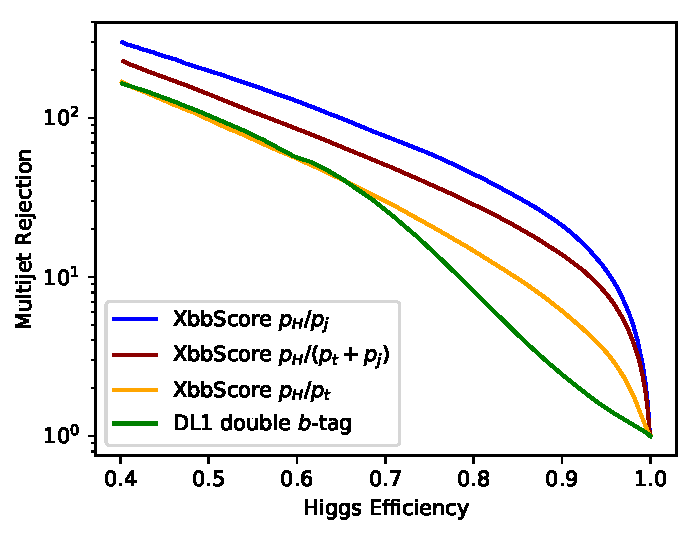
\includegraphics[width=0.4\textwidth]{appendices/figures/roc_multijet.pdf}
    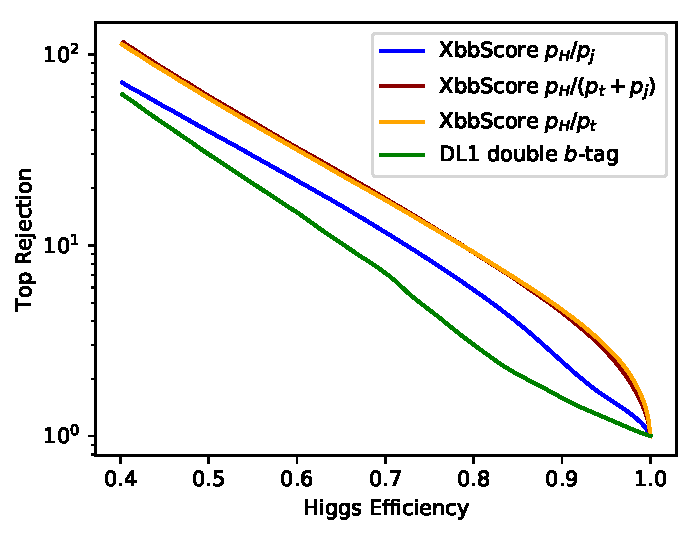
\includegraphics[width=0.4\textwidth]{appendices/figures/roc_top.pdf}
    \caption{ ROC plot: Comparison between different working points of CombinedXbbScore}
    \label{fig:roctop}
\end{figure}

\par The preliminary working points of the CombinedXbbScore are listed in Table.\ref{tab:combxbb}.

\begin{table}
    \footnotesize{
        \begin{center}
            \begin{tabular}{ c |c |c |c}
                \hline
                \hline
                Higgs efficiency [\%] & mixing fraction (f) & cut value \\
                50 & 0 & 5.1 \\
                60 & 0 & 4.8 \\
                70 & 0 & 3.9 \\
                50 & 0.2 & 4.5 \\
                60 & 0.2 & 3.9 \\
                70 & 0.2 & 3.0 \\
                50 & 1 & 3.6 \\
                60 & 1 & 3.0 \\
                70 & 1 & 2.1 \\
                \hline
                \hline
            \end{tabular}
        \end{center}
        }
    \caption{Preliminary working points of CombinedXbbScore}
    \label{tab:combxbb}
\end{table}

\section{Signal selection in Merged region using CombinedXbbScore}

\par For the merged region, instead of requiring two b-tagged VR track jets with 77\% working point as described in Section.\ref{sec:ana-sig:physobj}, cutting on the CombinedXbbScore of a large-R jet can choose the Xbb jets directly.
The background large-R jets (R = 1.0) is suppressed by applying a cut on CombinedXbbScore. 
To have a fair comparison within these two methods, 77\% working point is chosen for the VR track jets b-tagging and 60\% working points are chosen for the CombinedXbbScore tagger with different mixing fractions for all plots showed in this chapter.                    

\par The large-R jet mass distribution of the Z’+2HDM signal with $m_Z’ = 2800~GeV$ and $m_A = 300~GeV$ is scaled by a factor of 1000 and compared to backgrounds in both Fig.\ref{fig:mj_before} and Fig.\ref{fig:mj_after}.   

\par The left plot in Fig.\ref{fig:mj_before} shows the large-R jet mass distribution in the merged region while the right plot shows the large-R jet mass distribution after requiring two b-tagged VR track jets. 
Fig.\ref{fig:mj_before} shows the large-R jet mass distribution after applying cutting on CombinedXbbScore with mixing fraction $f=1$ (left) and $f=0$ (right).     

\begin{figure}[h]
    \centering
    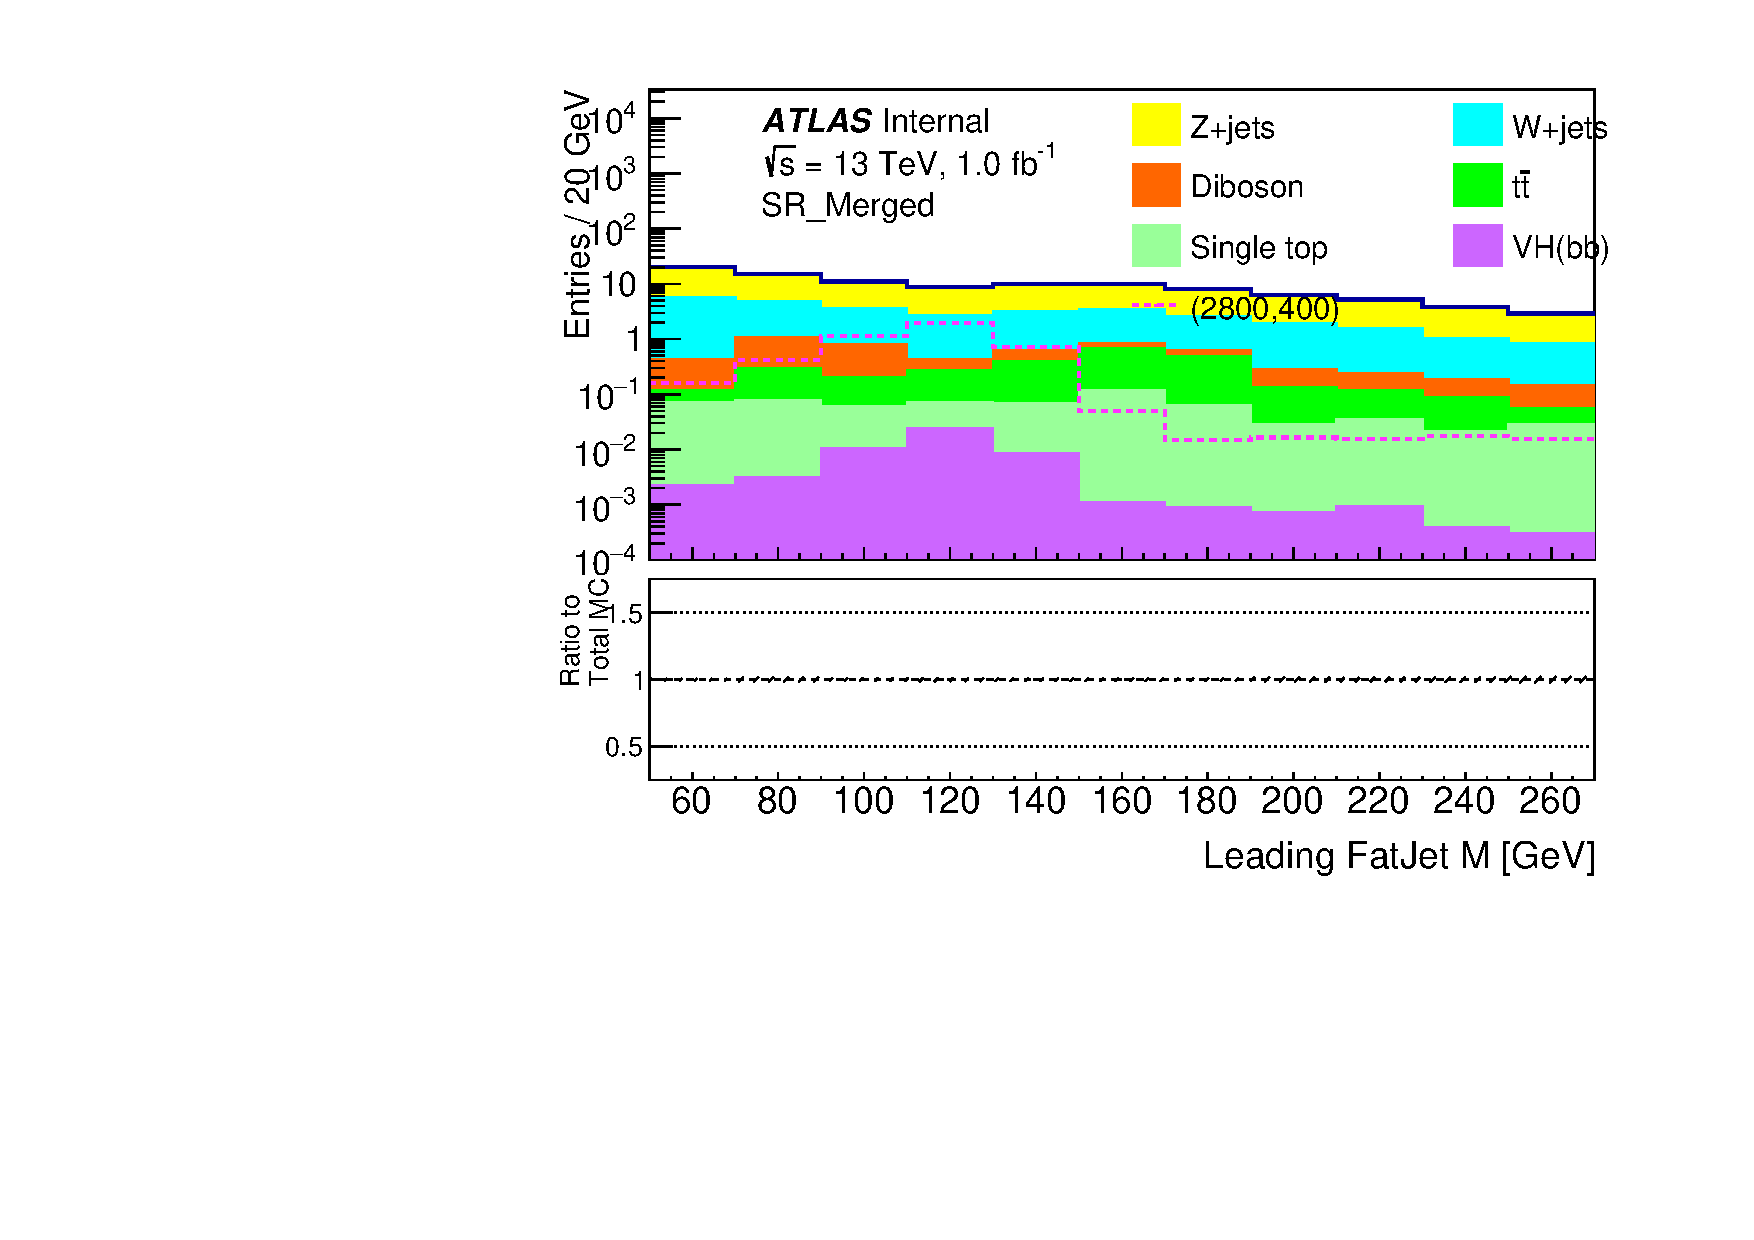
\includegraphics[width=0.4\textwidth]{appendices/figures/MC_MonoH_Nominal_SR_Merged_fatjets_m1_20GeV_LogY.pdf}
    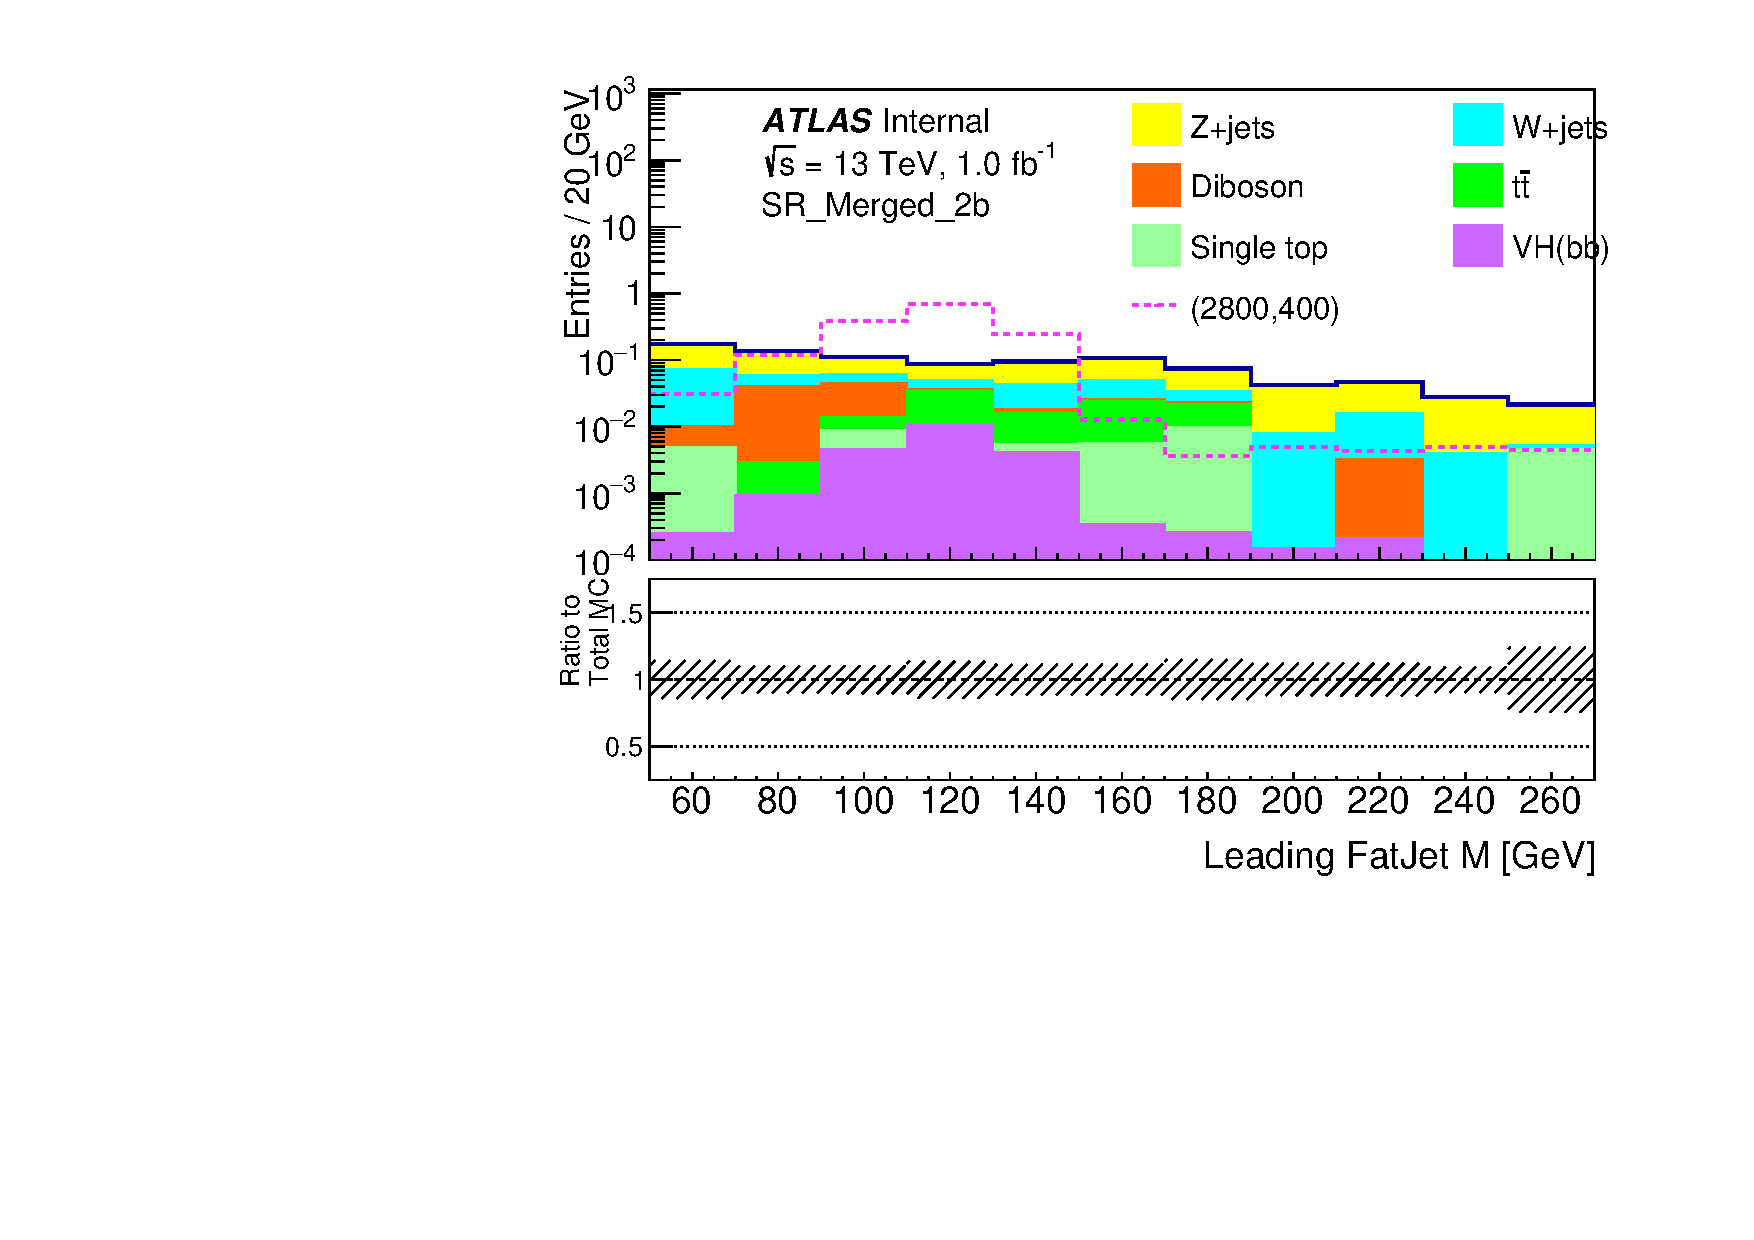
\includegraphics[width=0.4\textwidth]{appendices/figures/MC_MonoH_Nominal_SR_Merged_2b_fatjets_m1_20GeV_LogY_vr.pdf}
    \caption{Leading Fatjet mass in Merged region (left) and 2b Merged region defined by 2-b tagged VR (right)}
    \label{fig:mj_before}
\end{figure}

\begin{figure}[h]
    \centering
    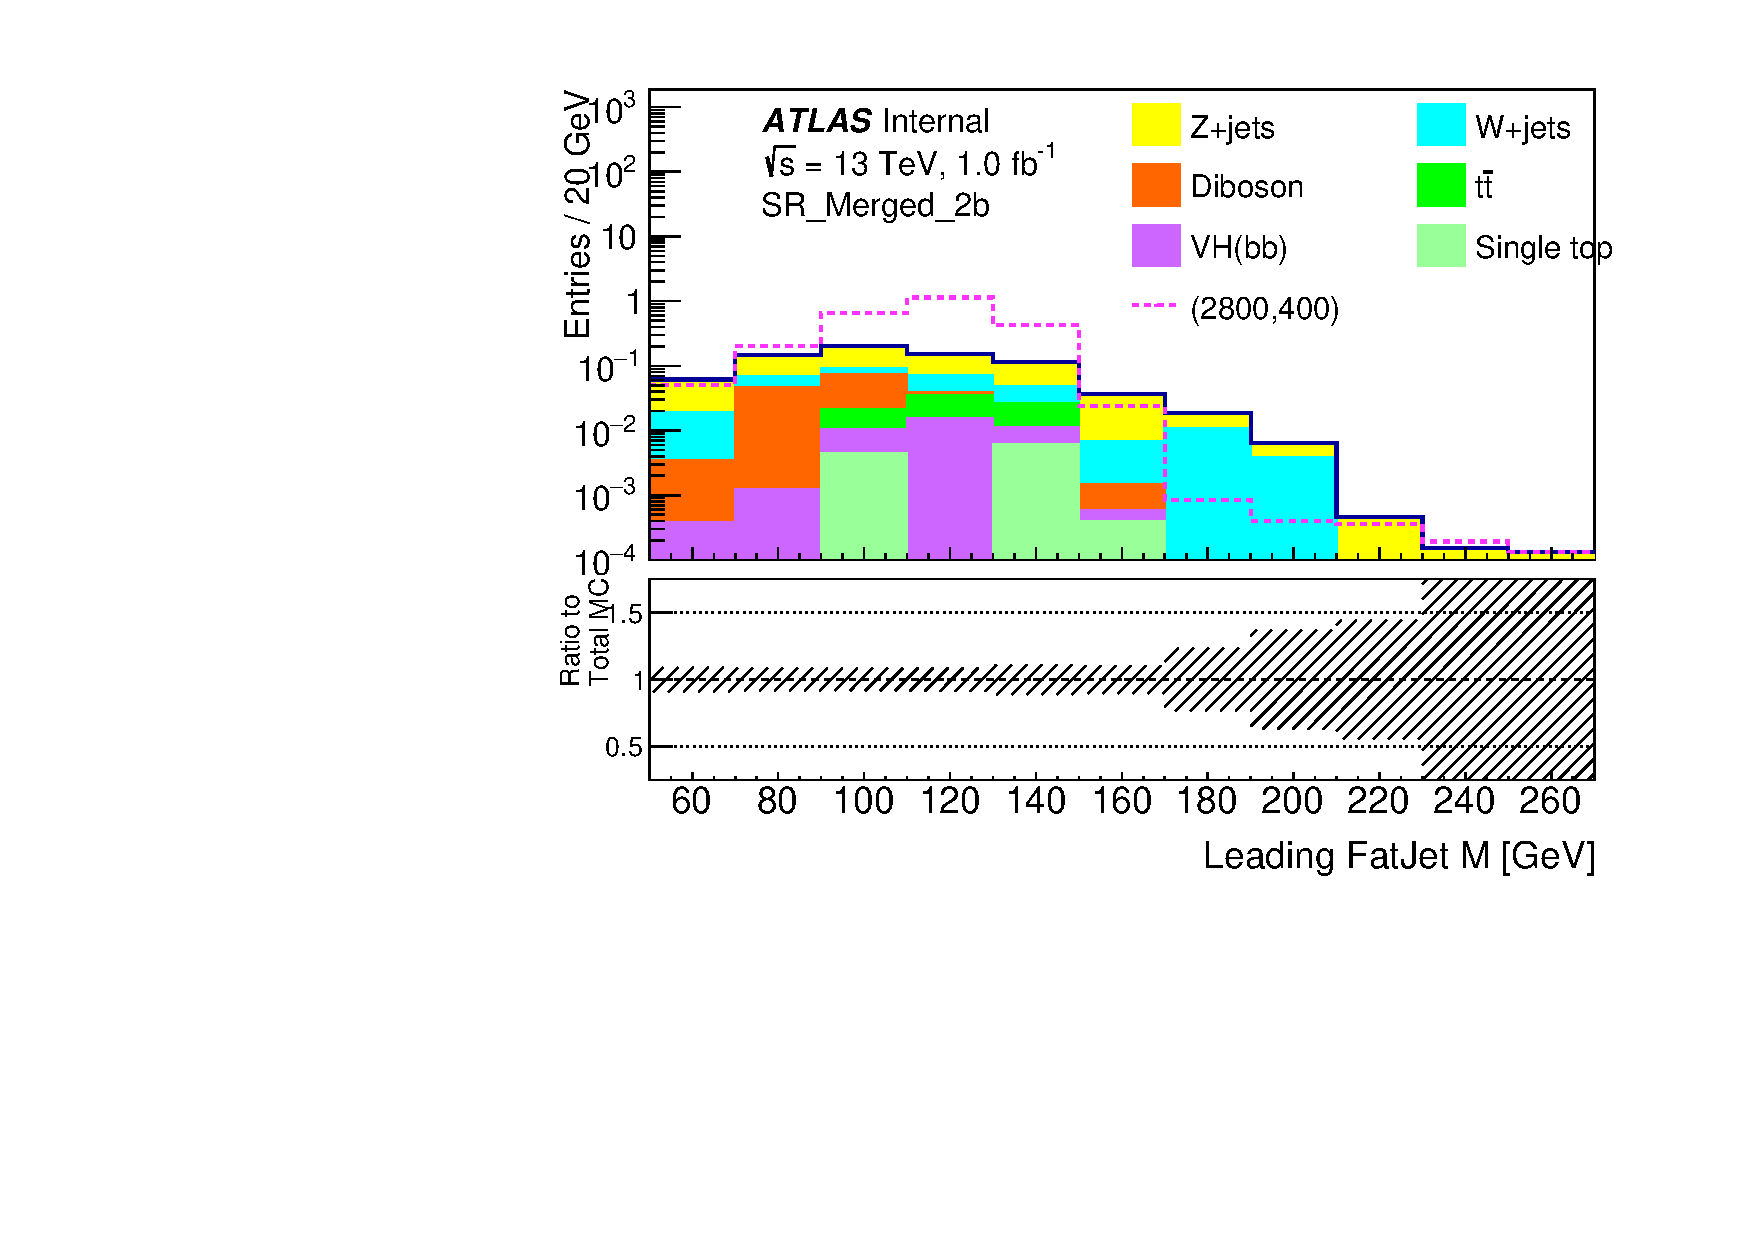
\includegraphics[width=0.4\textwidth]{appendices/figures/MC_MonoH_Nominal_SR_Merged_2b_fatjets_m1_20GeV_LogY_xbb.pdf}
    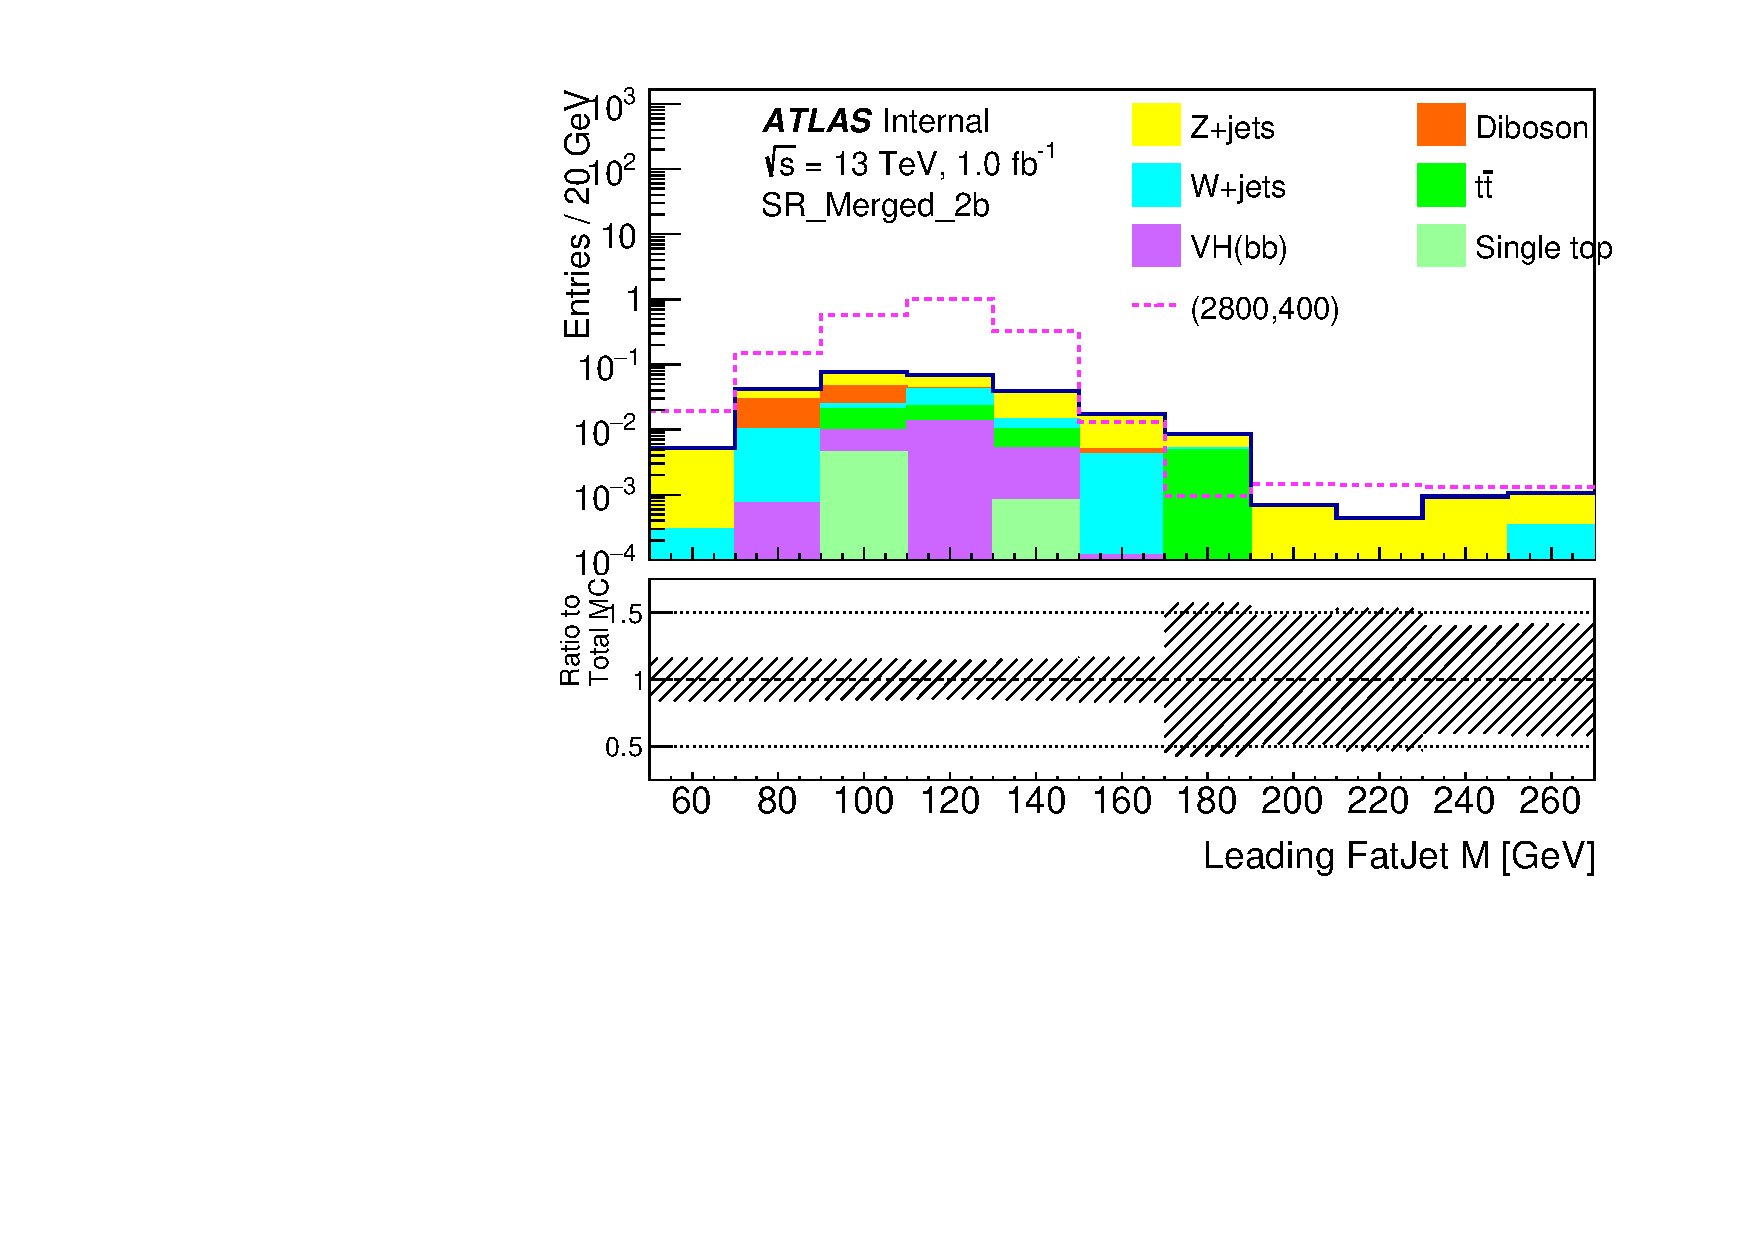
\includegraphics[width=0.4\textwidth]{appendices/figures/MC_MonoH_Nominal_SR_Merged_2b_fatjets_m1_20GeV_LogY_xbb_f0.pdf}
    \caption{Leading Fatjet mass in 2b Merged region defined by CombinedXbbScore}
    \label{fig:mj_after}
\end{figure}

\par While the CombinedXbbScore tagger did a much better job at suppressing backgrounds, it also shaped the background distributions. 

\subsection{Backgrounds breakdown of signal region and control regions}

\par To study the modeling and systematics, truth labeling is implemented in ntuples based on the truth particles ghost-associated to the large-R jets.
And the composition of the background on the 1L/2L control regions is examined.

\par Fig.\ref{fig:fl_mj} shows the large-R jet mass distribution in the 2b-tagged signal and control regions defined by the CombinedXbbScore.

\begin{figure}[h]
    \centering
    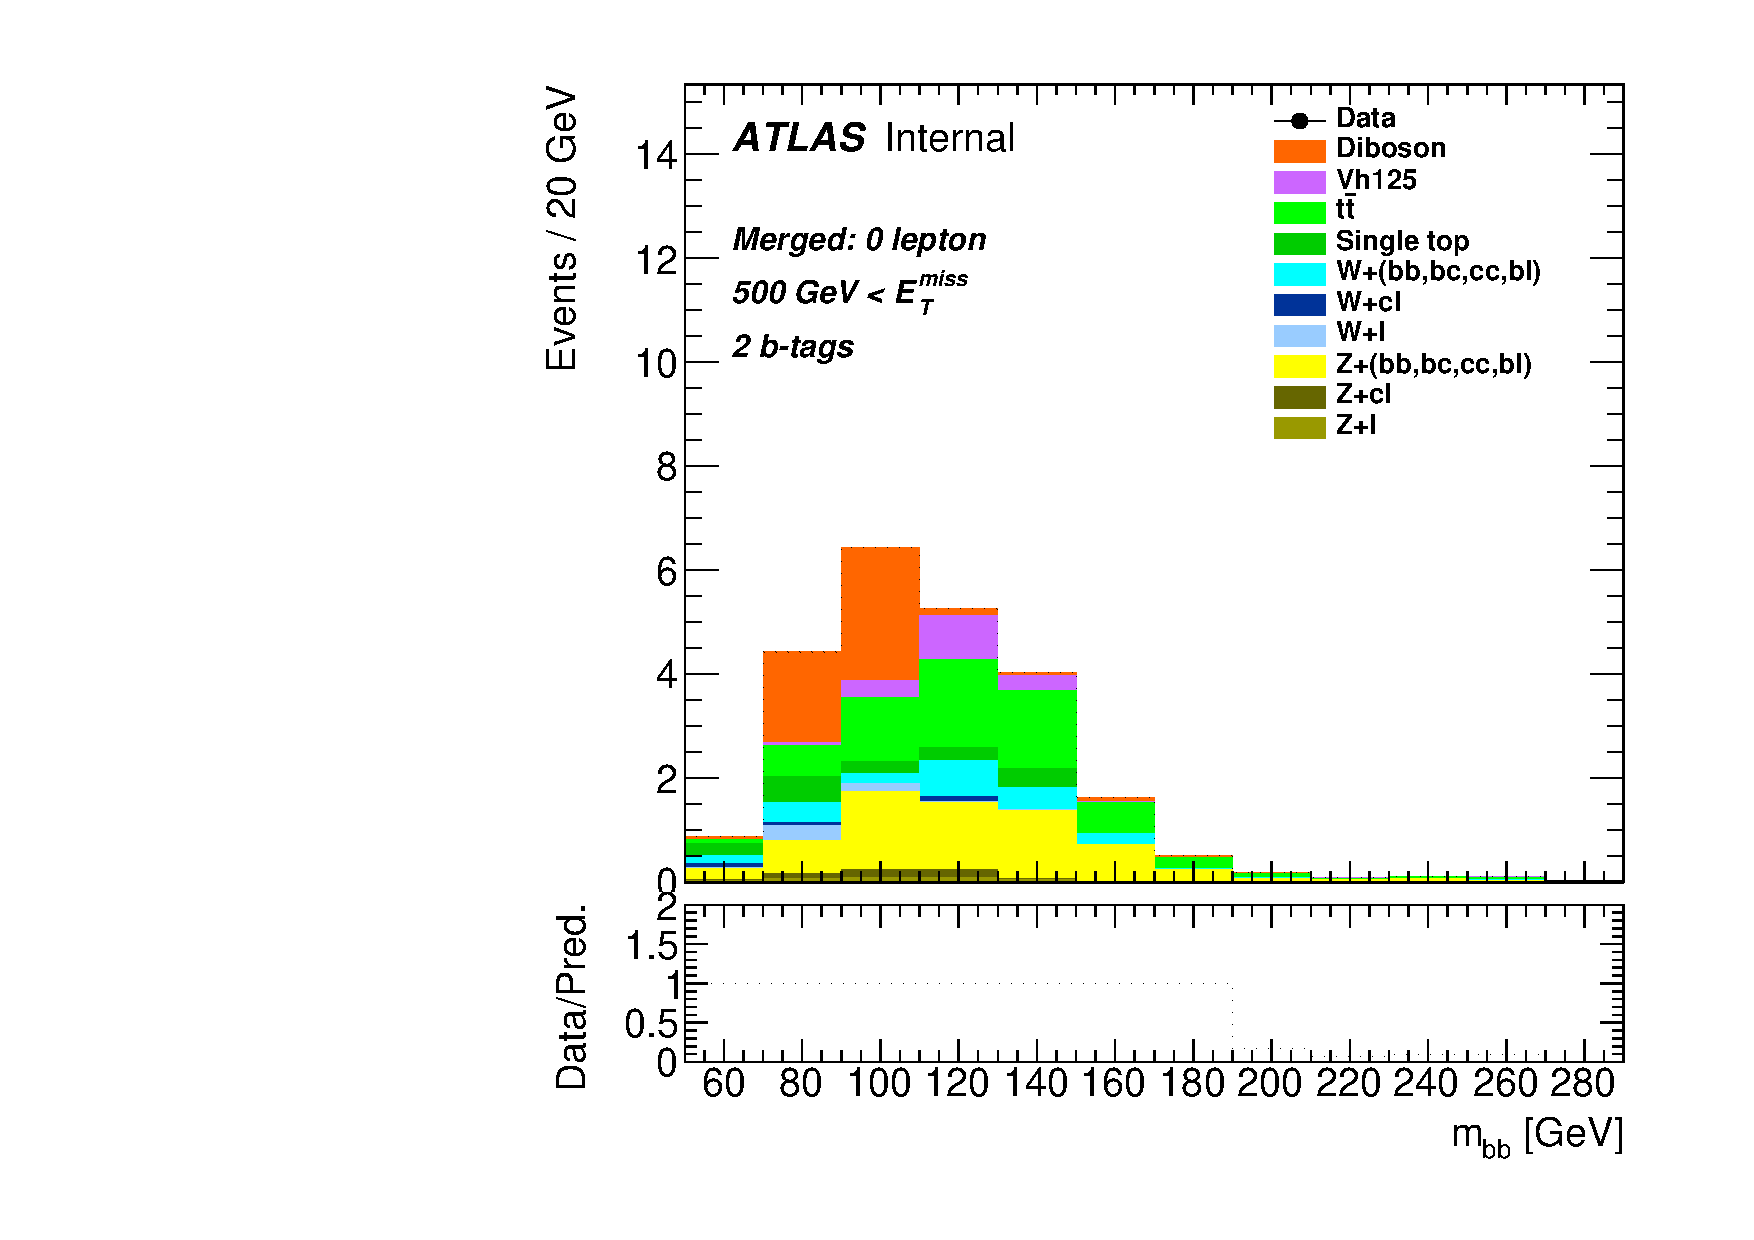
\includegraphics[width=0.4\textwidth]{appendices/figures/Region_BMin500_incFat1_Fat1_incJet1_Y2015_DSR_T2_L0_distmBB_J0_Prefit.pdf}
    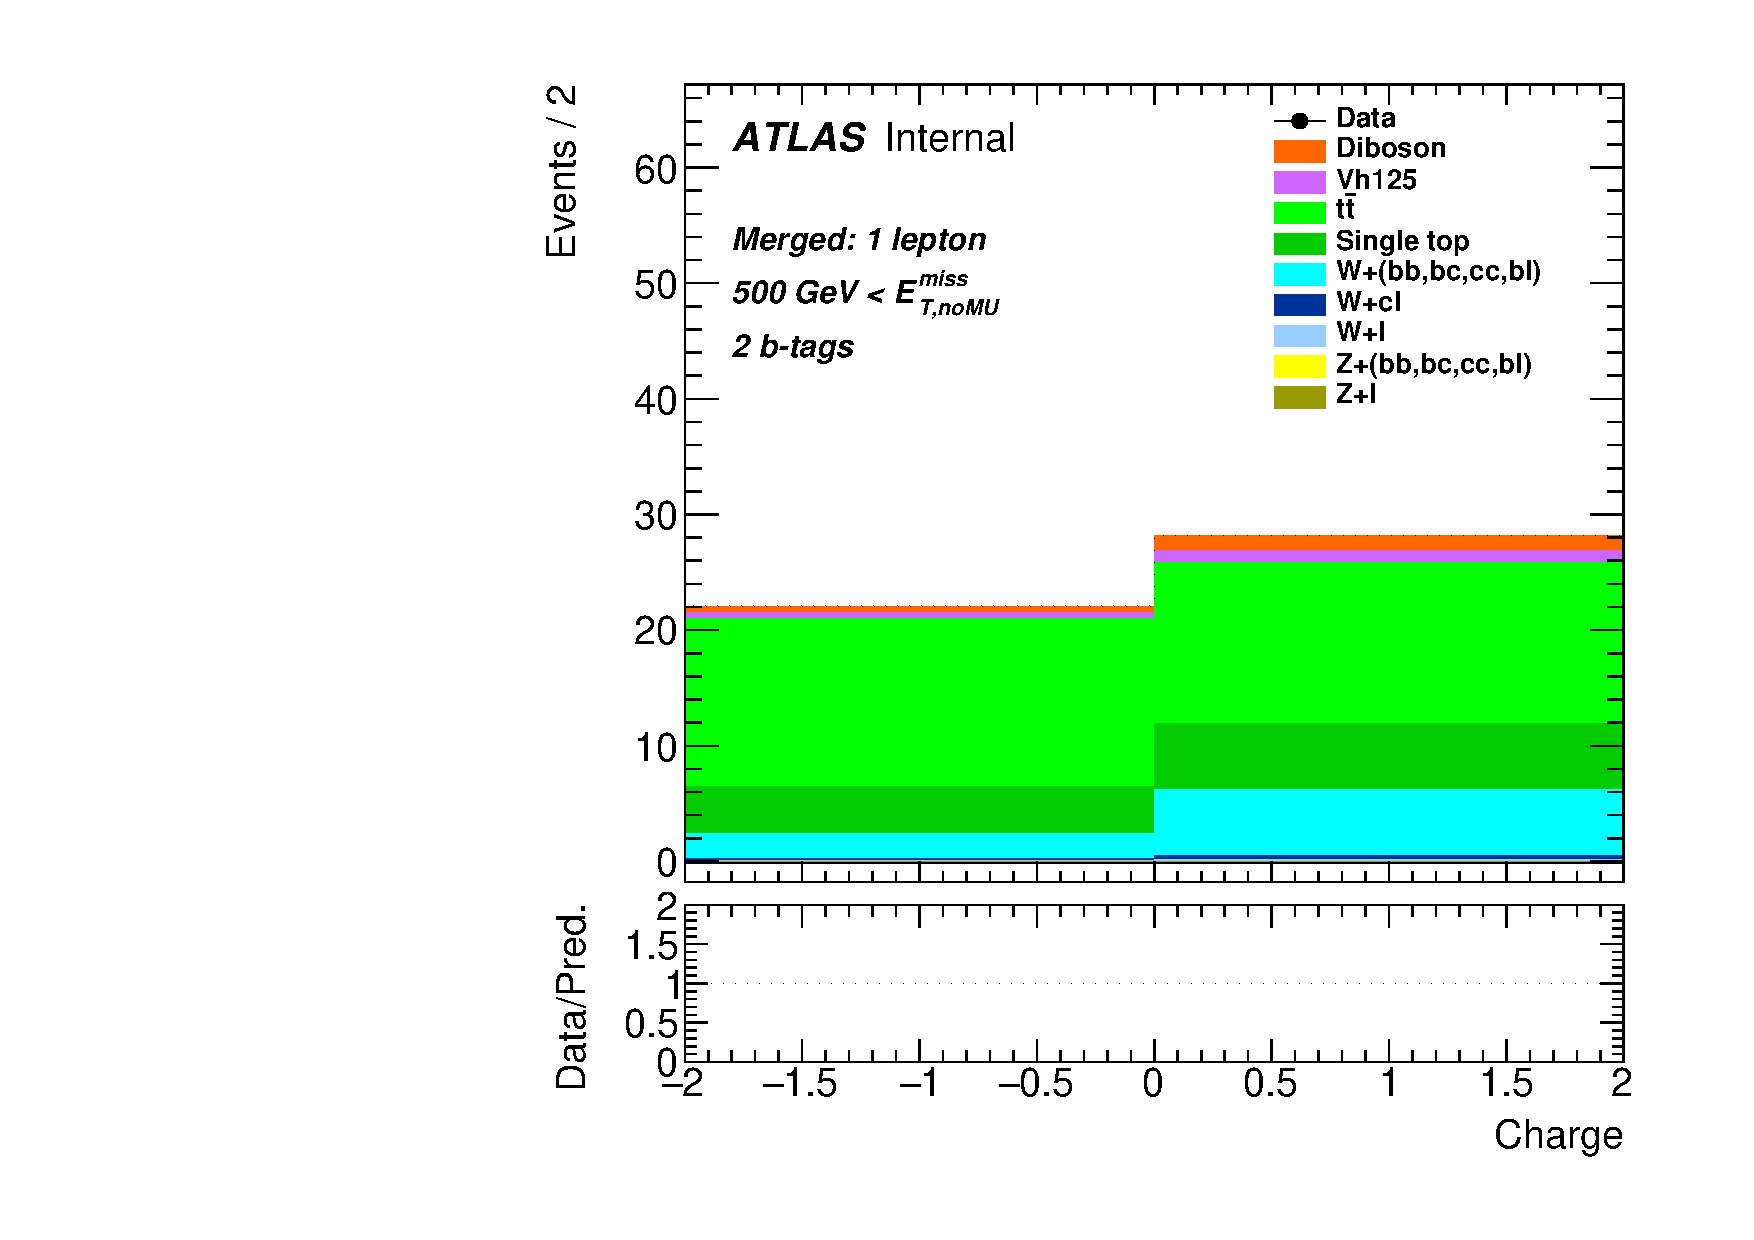
\includegraphics[width=0.4\textwidth]{appendices/figures/Region_BMin500_incFat1_Fat1_incJet1_Y2015_DCR1_T2_L1_distCharge_J0_Prefit.pdf}
    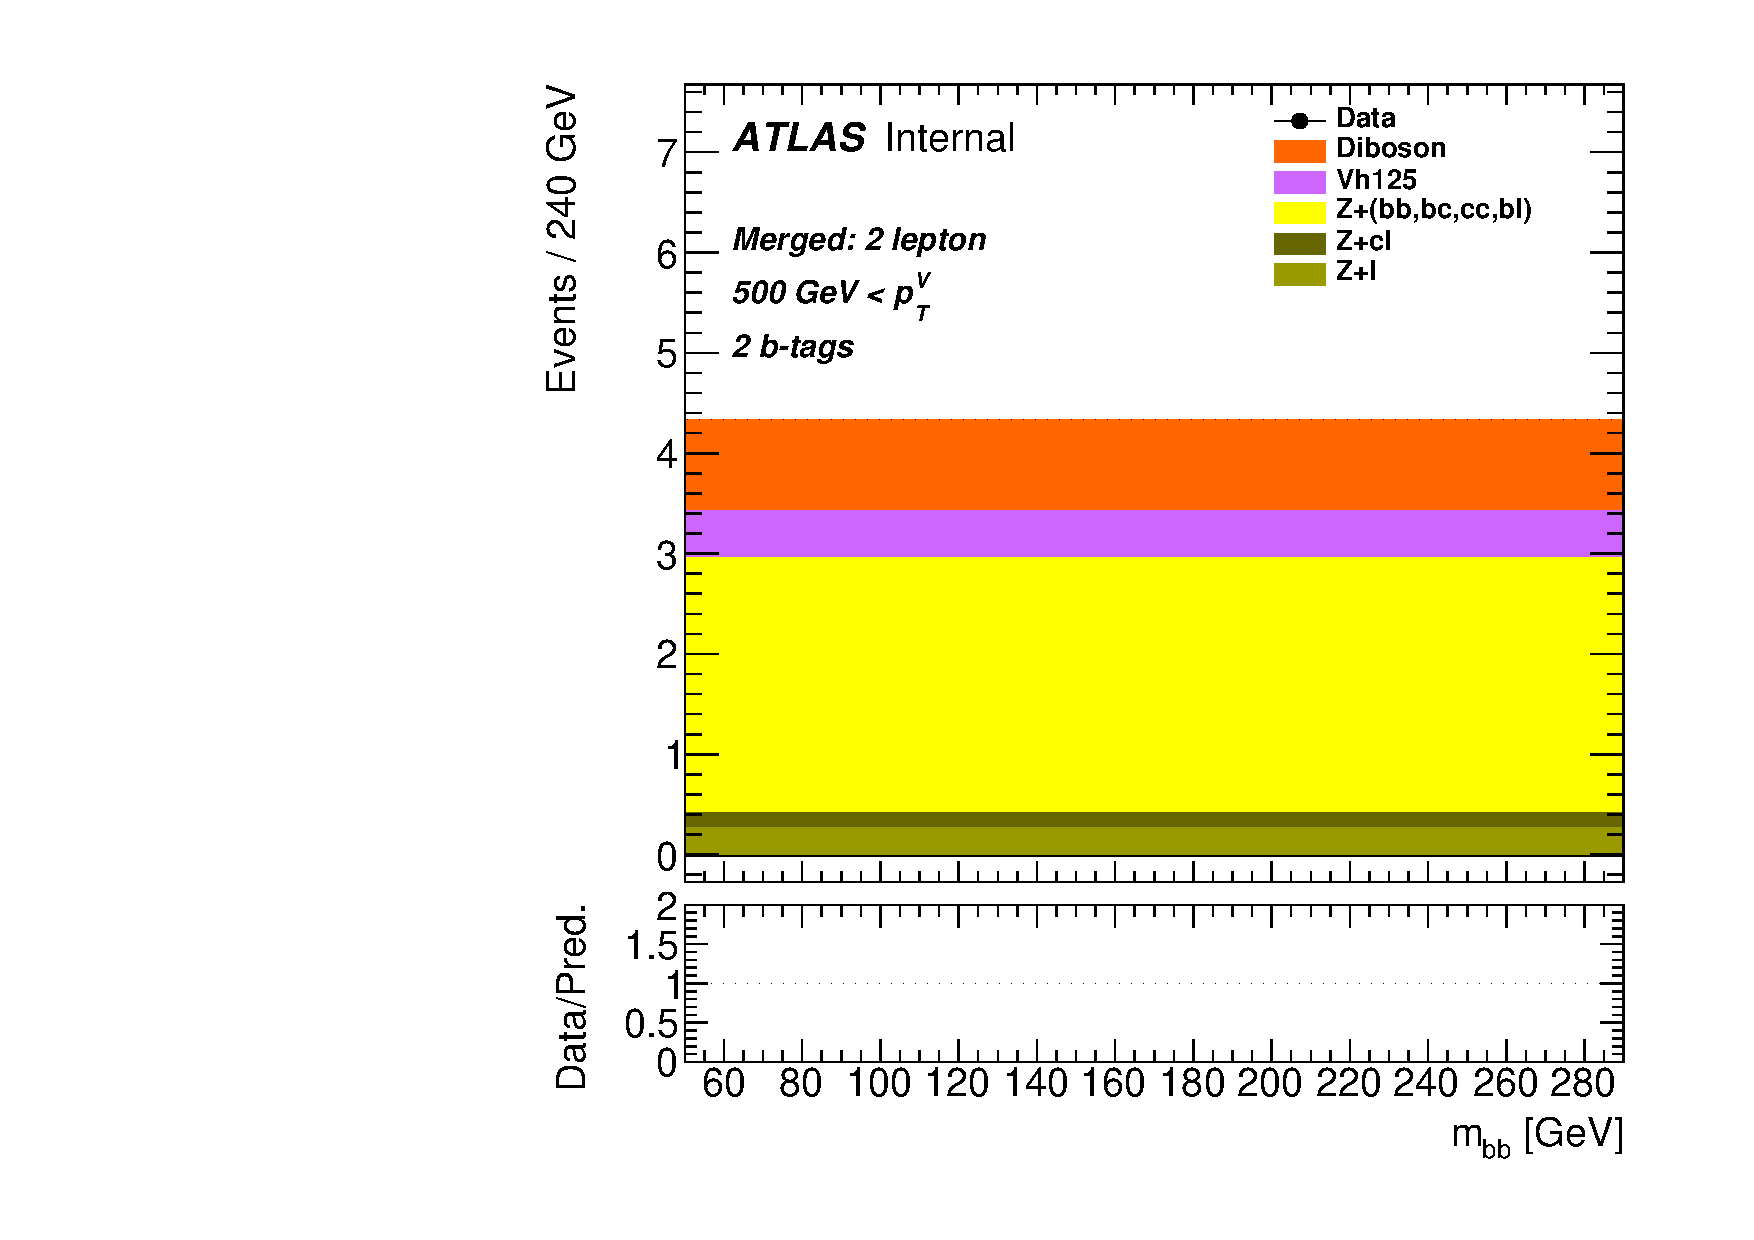
\includegraphics[width=0.4\textwidth]{appendices/figures/Region_BMin500_incFat1_Fat1_incJet1_Y2015_DCR2_T2_L2_distmBB_J0_Prefit.pdf}
    \caption{Large-R jet mass distribution in the 2-btagged signal and control regions.}
    \label{fig:fl_mj}
\end{figure}

\par Ideally, large-R jets selected by cutting on CombinedXbbScore are likely to have two b-hadrons ghost-associated to them and have a truth labeling of bb.

\par To have a clear look at the fraction of large-R jets labeling, the Xbb tag fraction which refers to the fraction of large-R jets with labeling bb are examined for 1 lepton region with W+jets samples in Fig.\ref{fig:xbbw} and for 2 regions with Z+jets samples in Fig.\ref{fig:xbbz}.

\begin{figure}[h]
    \centering
    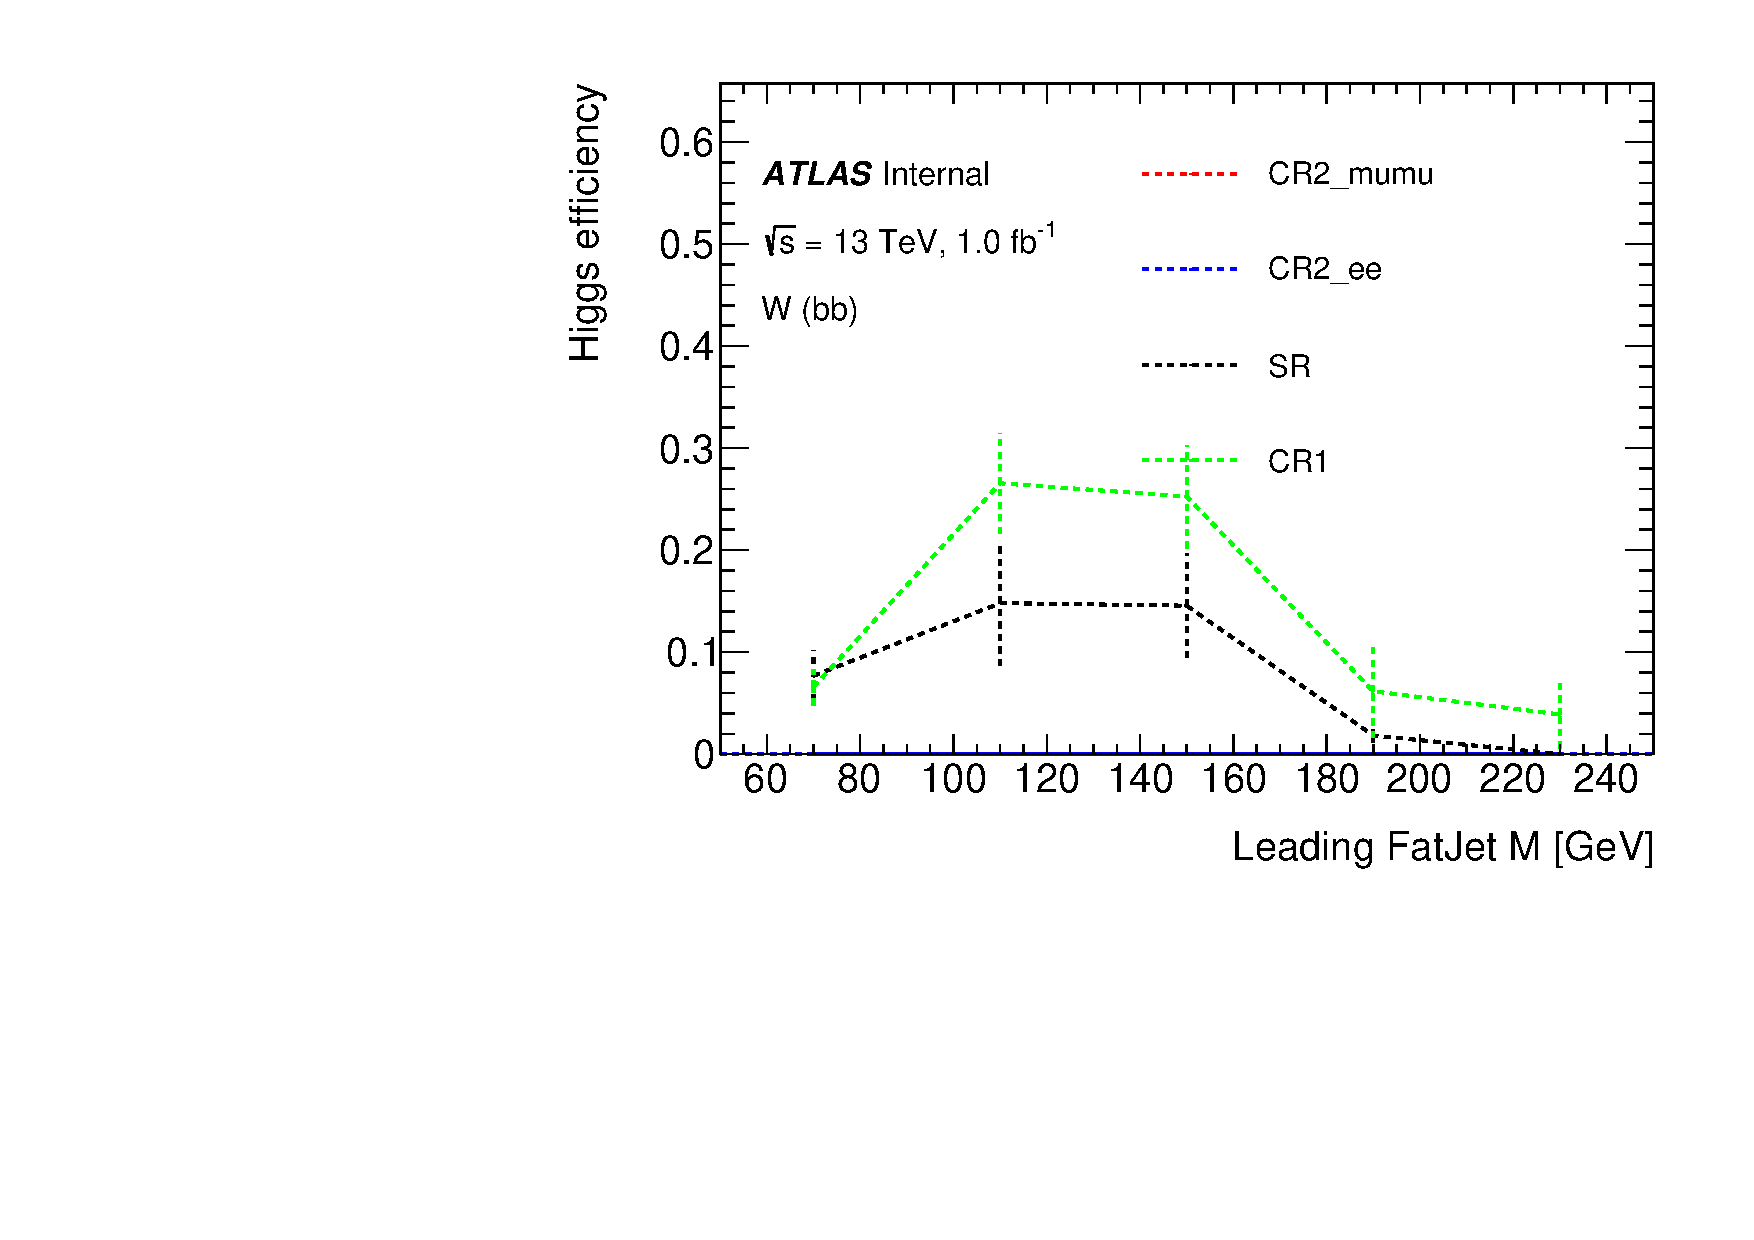
\includegraphics[width=0.45\textwidth]{appendices/figures/eff_W}
    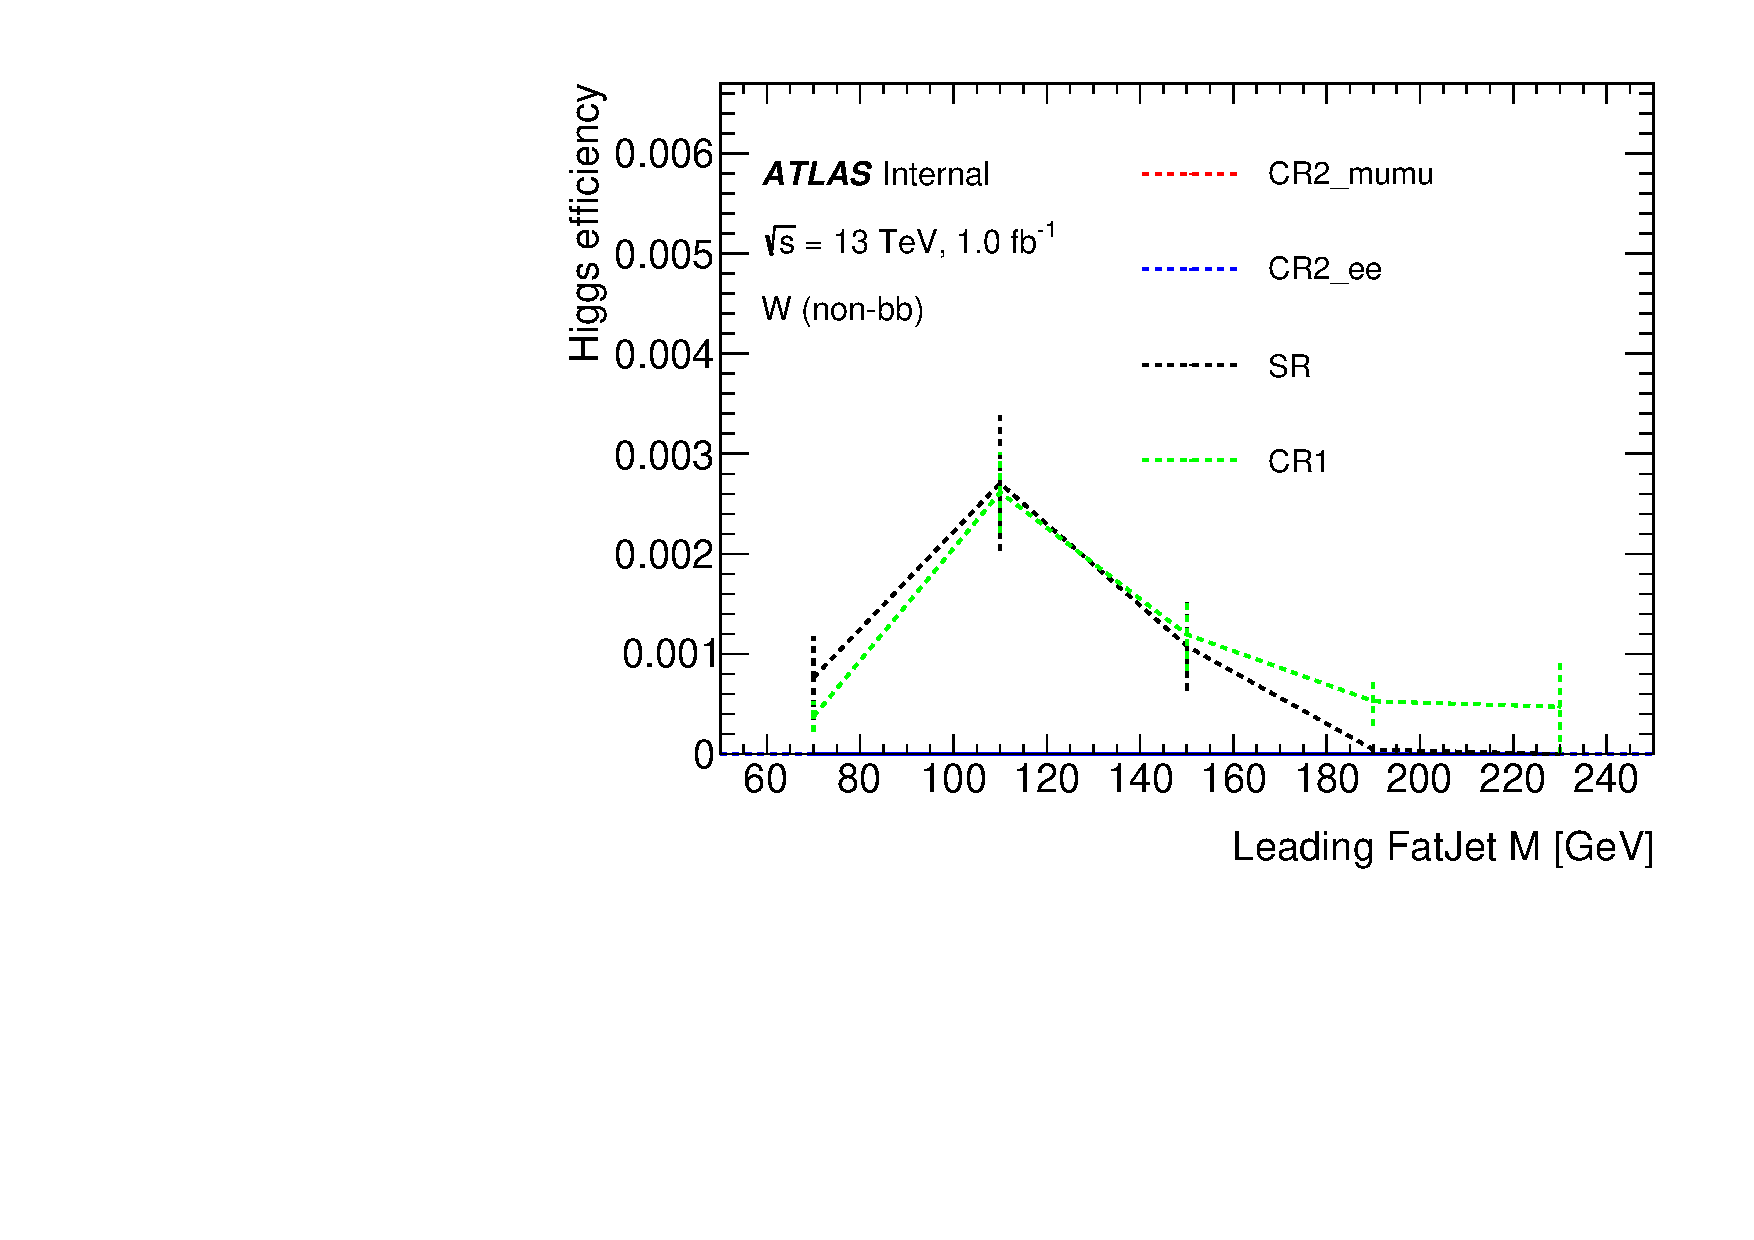
\includegraphics[width=0.45\textwidth]{appendices/figures/eff_Wnon}
    \caption{Fraction of large-R jets with bb labeling (left) and without bb labeling (right) in with W+jets samples.}
    \label{fig:xbbw}
\end{figure}

\begin{figure}[h]
    \centering
    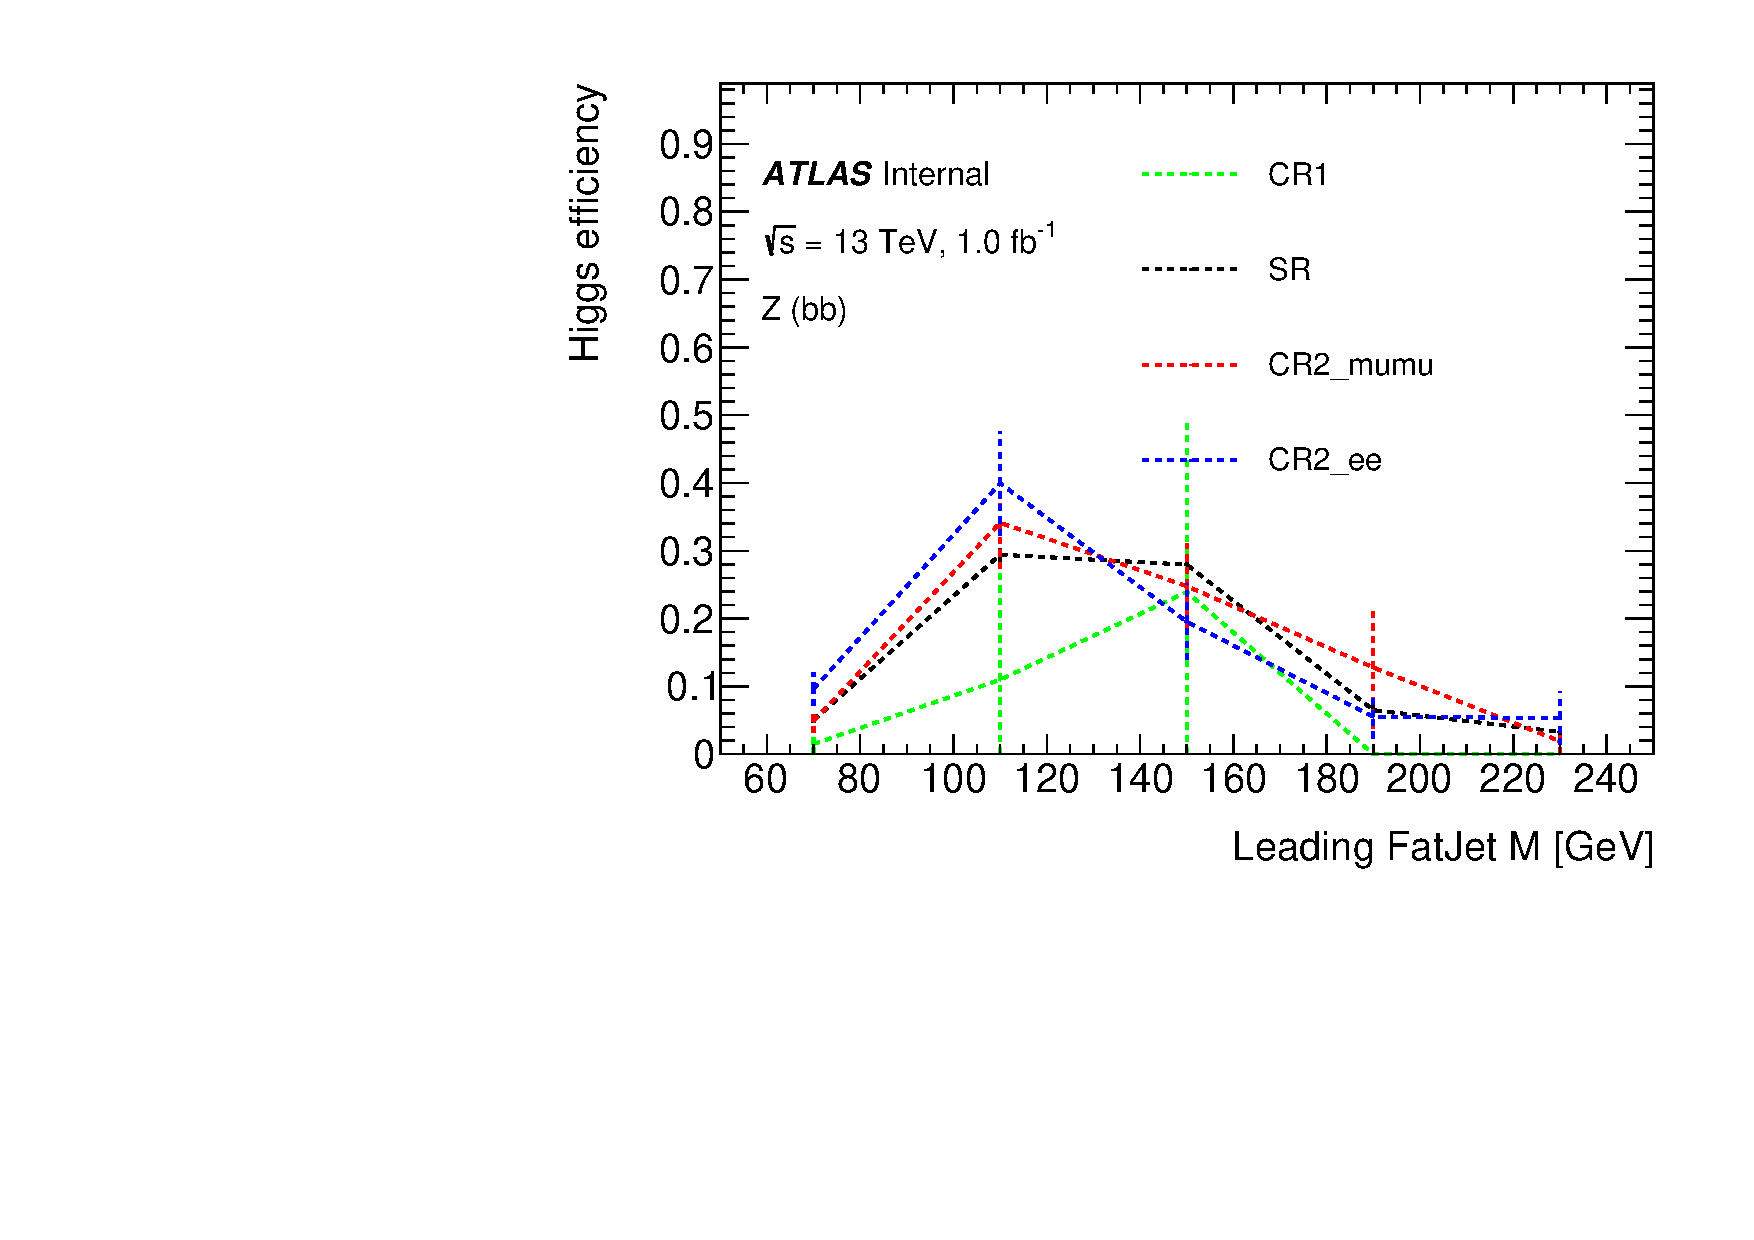
\includegraphics[width=0.45\textwidth]{appendices/figures/eff_Z}
    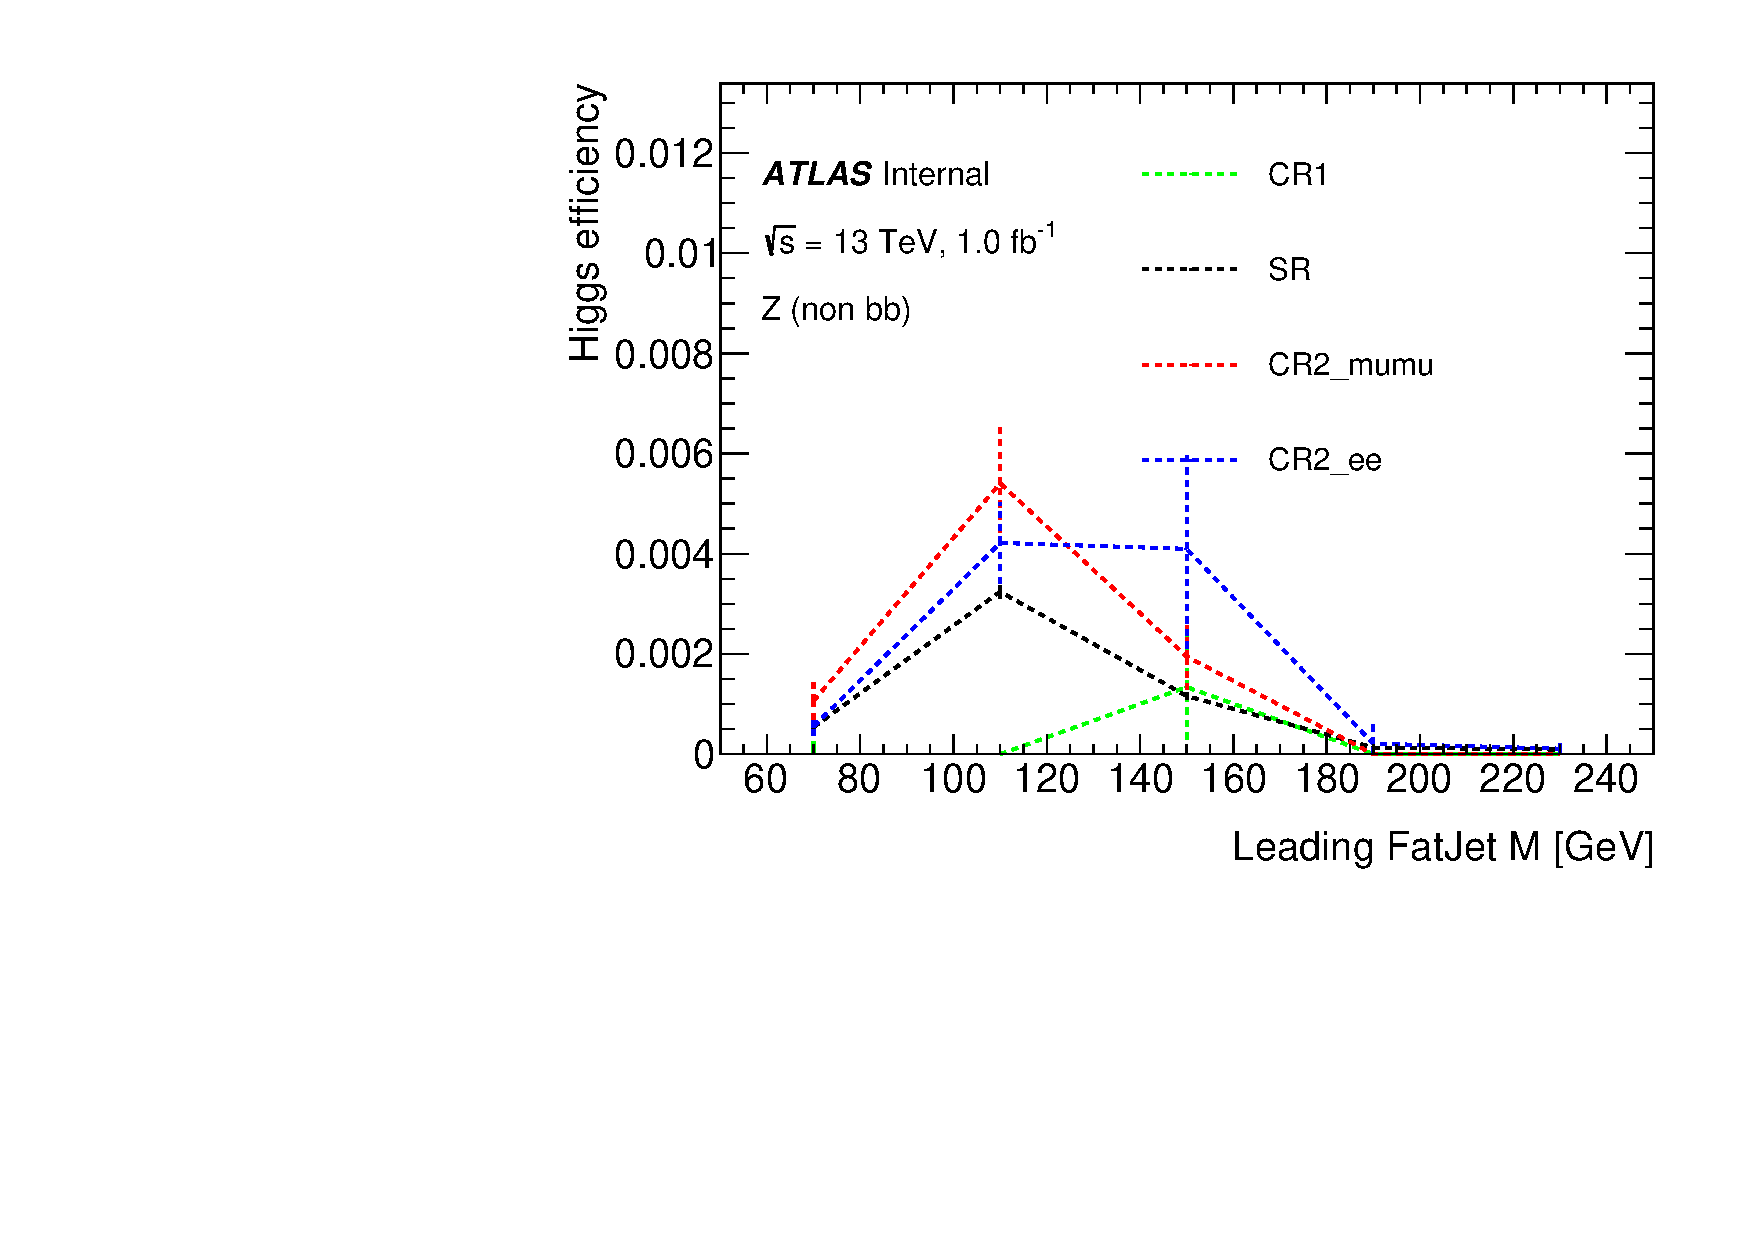
\includegraphics[width=0.45\textwidth]{appendices/figures/eff_Znon}
    \caption{Fraction of large-R jets with bb labeling (left) and without bb labeling (right) in with Z+jets samples.}
    \label{fig:xbbz}
\end{figure}

\par Xbb tag fraction of signal region vs 1b control regions in Fig.\ref{fig:xbbw} matches within uncertainty, as well as signal region vs 2b control regions in Fig.\ref{fig:xbbz}.
And the Xbb tag fraction peaks in around Higgs mass.

\par The flavor breakdown of backgrounds with truth labeling in signal and control regions is showed in Fig.\ref{fig:fl_pie}.

\begin{figure}[h]
    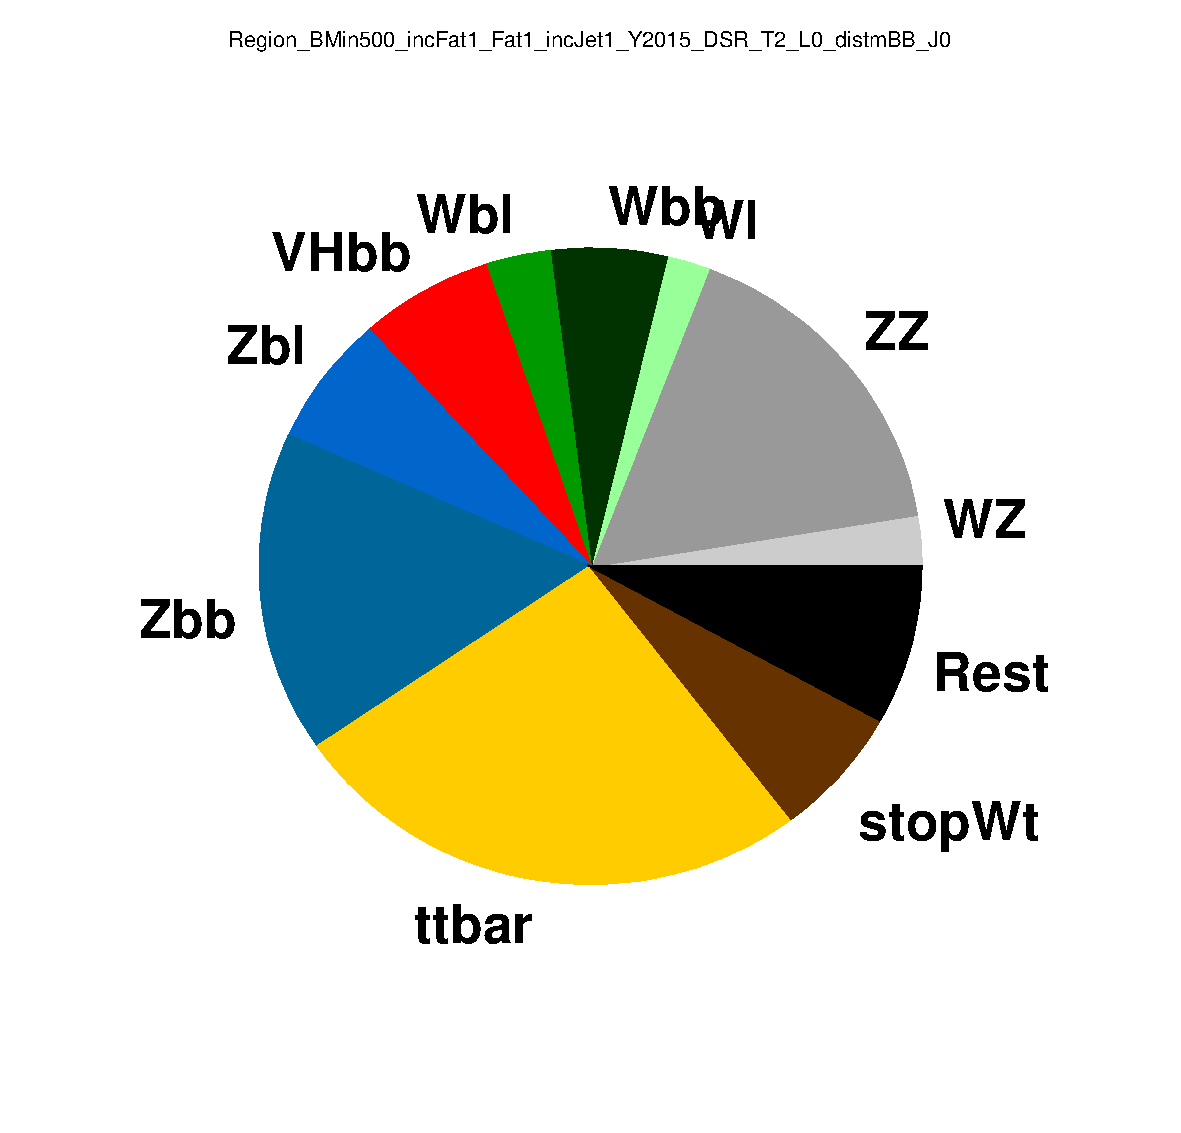
\includegraphics[ width=0.3\textwidth]{appendices/figures/pie0.pdf}
    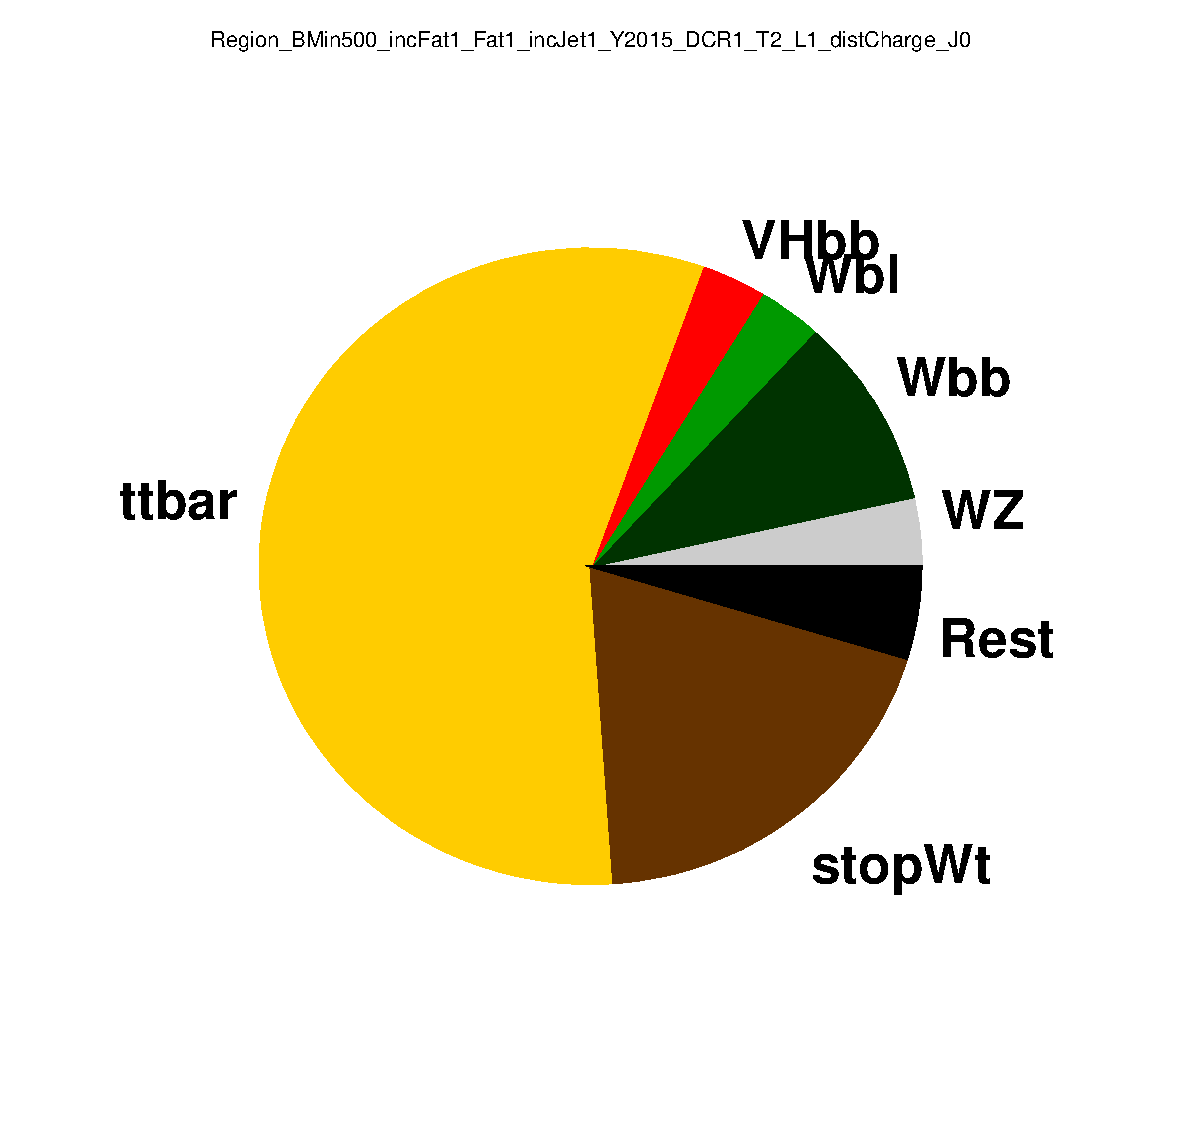
\includegraphics[ width=0.3\textwidth]{appendices/figures/pie1.pdf}
    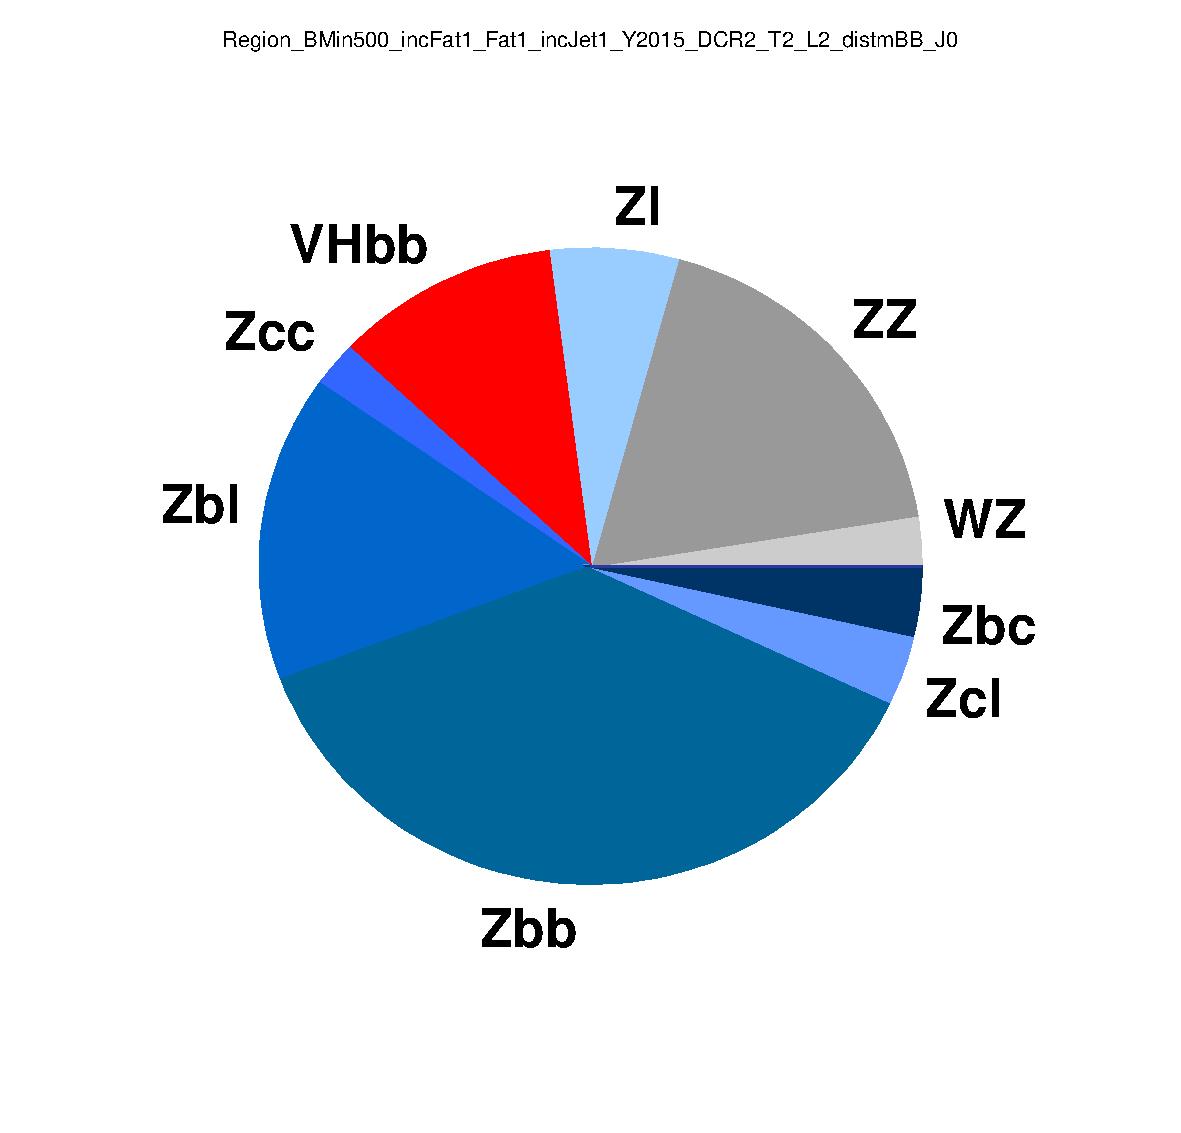
\includegraphics[ width=0.3\textwidth]{appendices/figures/pie2.pdf}
    \caption{Flavor breakdown of backgrounds with truth labeling in signal and control regions.}
    \label{fig:fl_pie}
\end{figure}

\par To further quantify the flavor breakdown in signal and control regions are showed in Table.\ref{tab:fl0}, Table.\ref{tab:fl1} and Table.\ref{tab:fl2}.

\begin{table}
    \centering
    \tiny
    \begin{tabular}{l|c|}
    \cline{2-2} & \multicolumn{1}{c|}{Zero lepton 2 tag merged,~$E_{T}^{miss}$$ >$ 500 GeV} \\
    \hline
    signal mzp1400\_mA600 & 0.0458$\pm$0.0005 \\
    \hline
    WZ    & 0.6106$\pm$0.2170 \\
    ZZ    & 3.9200$\pm$0.3486 \\
    Wl    & 0.4992$\pm$0.2104 \\
    Wcl   & 0.2709$\pm$0.0918 \\
    Wbb   & 1.3348$\pm$0.2478 \\
    Wbl   & 0.7481$\pm$0.1999 \\
    Wbc   & 0.0100$\pm$0.0070 \\
    Zl    & 0.3124$\pm$0.0293 \\
    VHbb  & 1.5404$\pm$0.0162 \\
    WW    & 0.1818$\pm$0.1285 \\
    Zcc   & 0.3775$\pm$0.0293 \\
    Zbl   & 1.5497$\pm$0.0580 \\
    Zbb   & 3.8587$\pm$0.0879 \\
    Zcl   & 0.4465$\pm$0.0431 \\
    Zbc   & 0.2807$\pm$0.0233 \\
    ttbar & 6.0874$\pm$0.2225 \\
    stopWt& 1.5491$\pm$0.4528 \\
    stops & 0.0200$\pm$0.0141 \\
    \hline
    Total Bkgd & 23.5977$\pm$3.3084 \\
    \hline
    \end{tabular}
    \caption{Flavor breakdown of backgrounds with truth labeling in signal region.}
    \label{tab:fl0}
\end{table}

\begin{table}
    \centering
    \tiny
    \begin{tabular}{l|c|}
        \cline{2-2} & \multicolumn{1}{c|}{One lepton 2 tag merged,~$E_{T}^{miss}$$ >$ 500 GeV} \\
        \hline
        WZ    & 1.7570$\pm$0.2641 \\
        ZZ    & 0.0775$\pm$0.0264 \\
        Wl    & 0.2212$\pm$0.0978 \\
        Wcl   & 0.5467$\pm$0.2127 \\
        Wbb   & 4.8836$\pm$0.5282 \\
        Wcc   & 0.5283$\pm$0.1443 \\
        Wbl   & 1.5783$\pm$0.2929 \\
        Wbc   & 0.8691$\pm$0.2415 \\
        Zl    & 0.0060$\pm$0.0043 \\
        VHbb  & 1.5967$\pm$0.0162 \\
        Zbl   & 0.0093$\pm$0.0093 \\
        Zbb   & 0.0333$\pm$0.0276 \\
        ttbar & 28.449$\pm$0.8372 \\
        stopWt& 9.6438$\pm$1.1237 \\
        stops & 0.0704$\pm$0.0321 \\
        \hline
        Total Bkgd & 50.2699$\pm$3.1672 \\
        \hline
    \end{tabular}
    \caption{Flavor breakdown of backgrounds with truth labeling in 1 lepton control region.}
    \label{tab:fl1}
\end{table}    

\begin{table}
    \centering
    \tiny
    \begin{tabular}{l|c|}
        \cline{2-2} & \multicolumn{1}{c|}{Two lepton 2 tag merged, $E_{T}^{miss}$ $>$ 500 GeV} \\
        \hline
        WZ    & 0.1108$\pm$0.0427 \\
        ZZ    & 0.7880$\pm$0.1048 \\
        Zl    & 0.2722$\pm$0.1364 \\
        VHbb  & 0.4736$\pm$0.0053 \\
        Zcc   & 0.0991$\pm$0.0360 \\
        Zbl   & 0.6740$\pm$0.0969 \\
        Zbb   & 1.6105$\pm$0.1363 \\
        Zcl   & 0.1514$\pm$0.0428 \\
        Zbc   & 0.1524$\pm$0.0404 \\
        \hline
        Total Bkgd & 4.3320$\pm$ 5.8464 \\
        \hline
    \end{tabular}
    \caption{Flavor breakdown of backgrounds with truth labeling in 2 lepton control region.}
    \label{tab:fl2}
\end{table}

\par According to the tables above, the Wbb fraction in W+jets in the signal region is 46.62\% $\pm$ 10.76\% compared to 56.60\% $\pm$ 7.68\% in 1 lepton control region. 
And the Zbb fraction in Z+jets is 56.53\%$\pm$1.64\% compared to 54.42\%$\pm$6.21\% in 2 lepton control region.

\subsection{Preliminary significance study}

\par To quantify the improvement brought by the CombinedXbbScore, the signal significances of these two methods are compared.
Signal Significance in each bin is defined as
\begin{equation}
    S_i = \sqrt{2(s + b)ln(1 + \frac{s}{b}) − s},
\end{equation}
where s, b is the count of signal and background in the i-th bin.

\par And the Bin-by-bin signal significance is defined as
\begin{equation}
    S_{bin-by-bin} = \sqrt{\sum_i S_i^2}, 
\end{equation}

\par Fig.\ref{fig:ss_ratio} (left) shows the ratio of the signal significance of the 2b region defined by CombinedXbbScore vs 2b b-tagged VR track jets with the Higgs window [70, 140]~GeV,
while the right plot is without the Higgs window.
\begin{figure}[h]
    \centering
    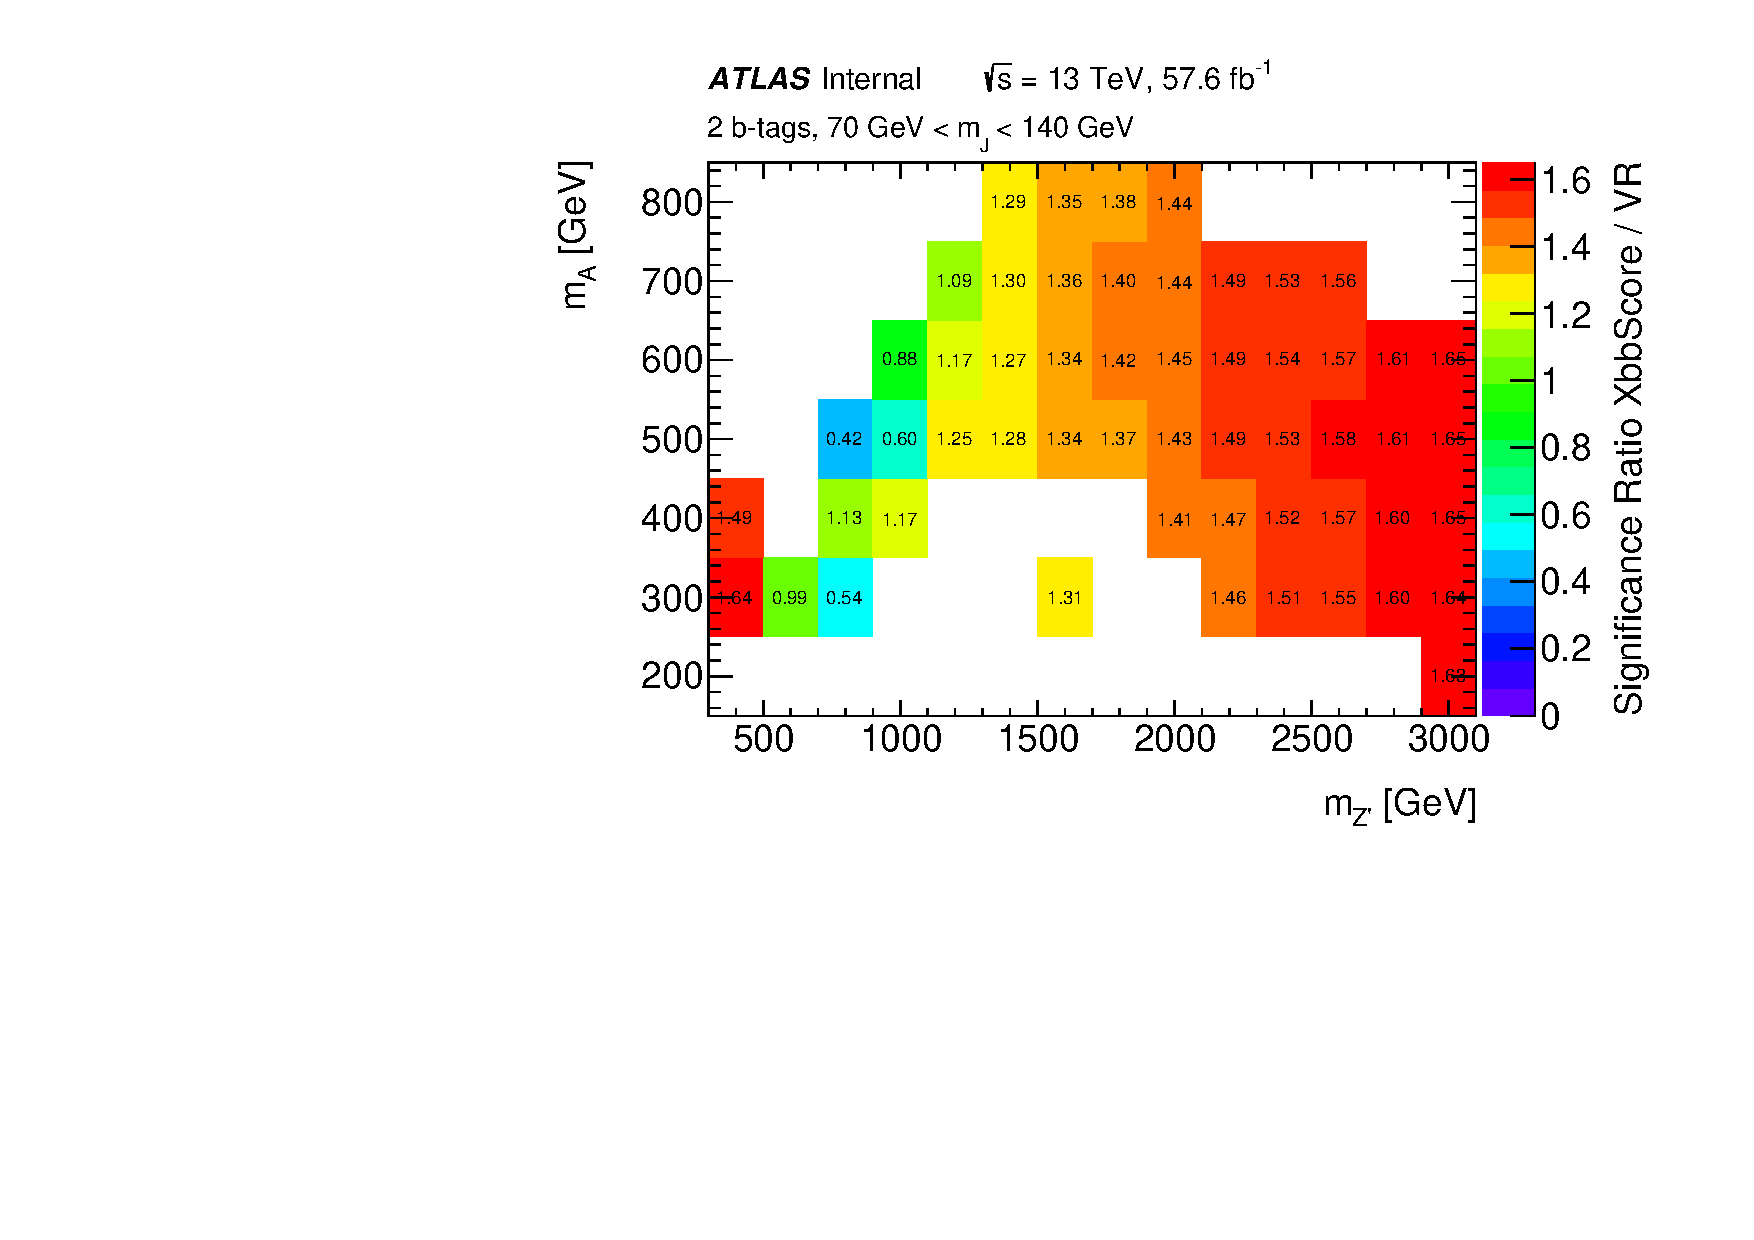
\includegraphics[width=0.45\textwidth]{appendices/figures/2b-tags_XbbScoreoverVR_HiggsWindow.pdf}
    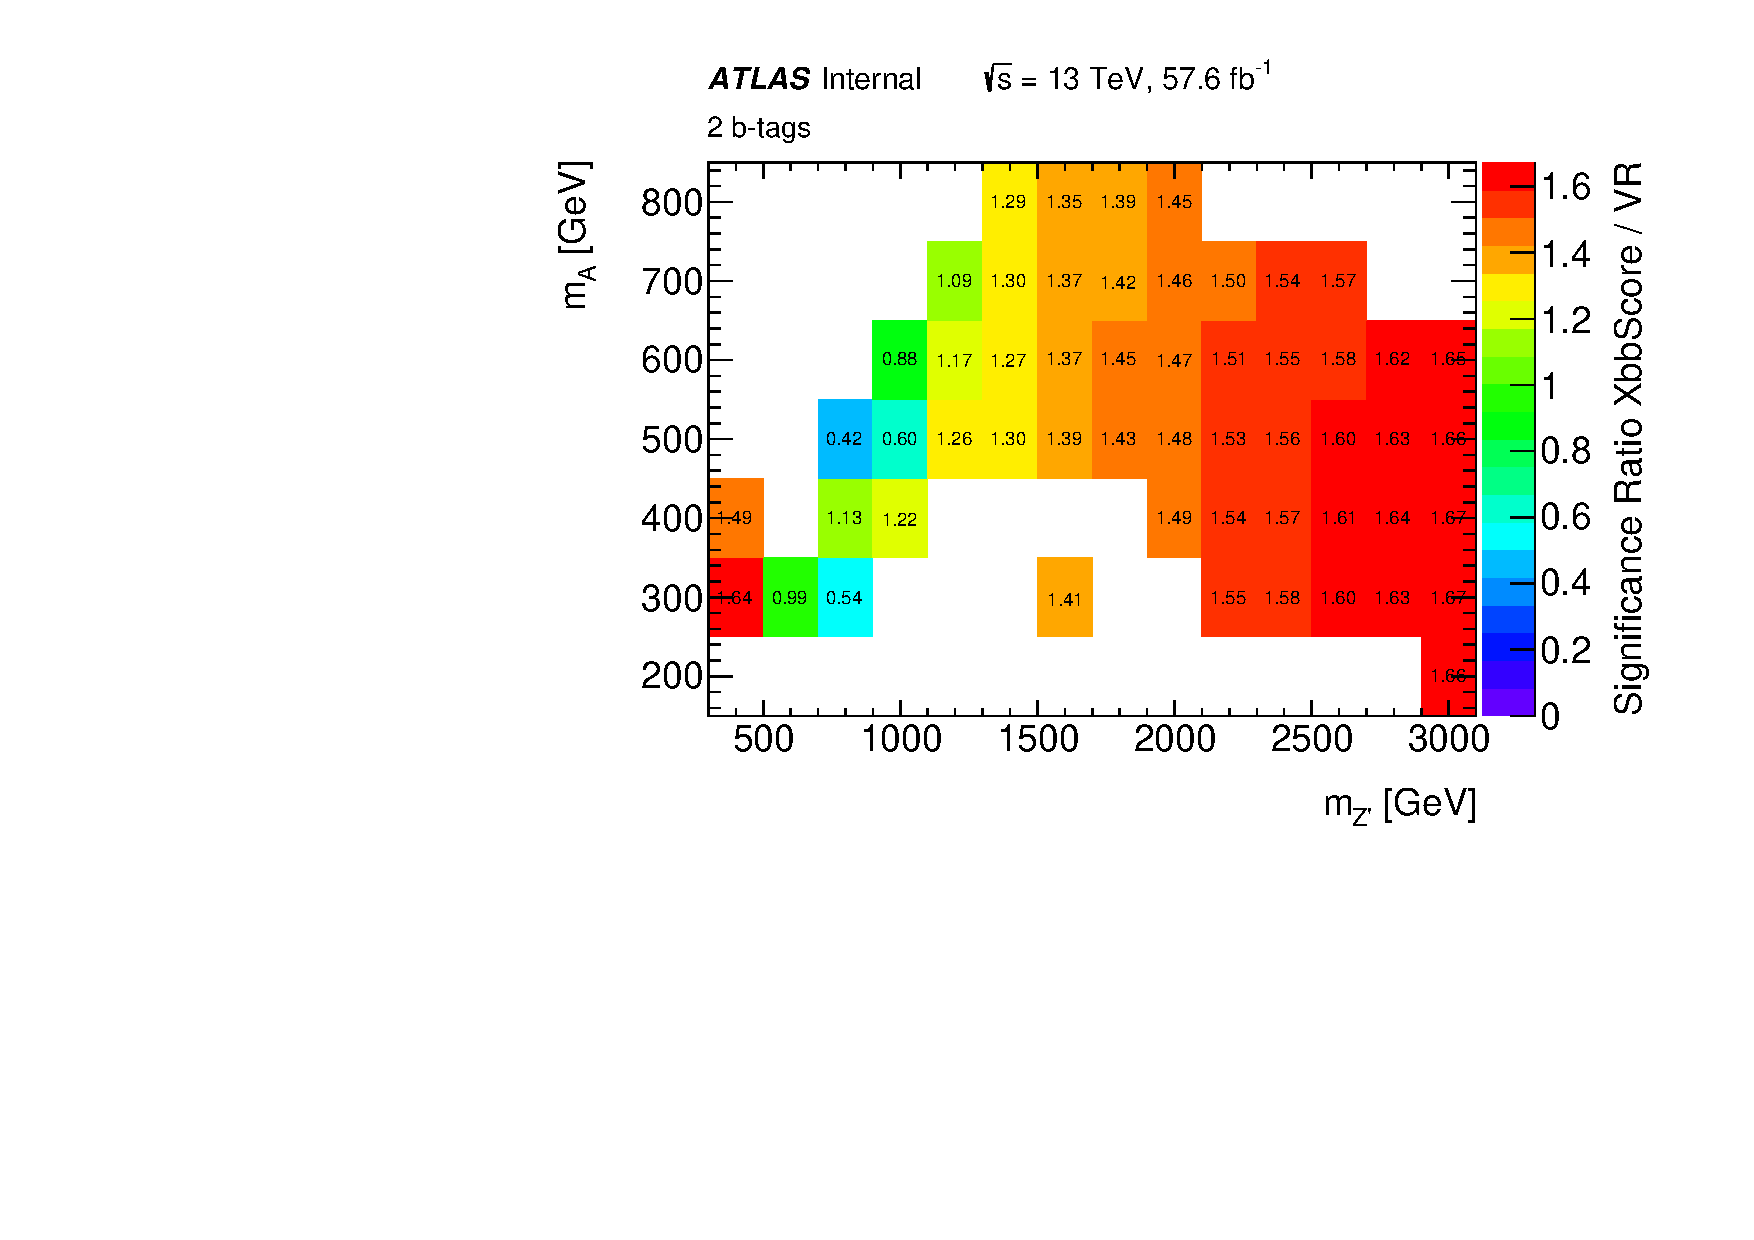
\includegraphics[width=0.45\textwidth]{appendices/figures/2b-tags_XbbScoreoverVR.pdf}
    \caption{Ratio of signal significance of 2b merged region defined by CombinedXbbScore compared to the original method with or without the Higgs window.}
    \label{fig:ss_ratio}
\end{figure}

\chapter{Analysis supplementary materials}

Sample text sample text sample text. Sample text sample text sample text.
Sample text sample text sample text. Sample text sample text sample text.
Sample text sample text sample text. Sample text sample text sample text.
Sample text sample text sample text. Sample text sample text sample text.
Sample text sample text sample text. Sample text sample text sample text.
Sample text sample text sample text. Sample text sample text sample text.

\section{$pp \rightarrow Hb\bar{b}$}
Sample text sample text sample text. Sample text sample text sample text.
Sample text sample text sample text. Sample text sample text sample text.
Sample text sample text sample text. Sample text sample text sample text.

\subsection{Sample subsection}
Sample text sample text sample text. Sample text sample text sample text.
Sample text sample text sample text. Sample text sample text sample text.
Sample text sample text sample text. Sample text sample text sample text.

\subsection{Sample subsubsection}
Sample text sample text sample text. Sample text sample text sample text.
Sample text sample text sample text. Sample text sample text sample text.
Sample text sample text sample text. Sample text sample text sample text.

\section{$pp \rightarrow q\bar{q}b\bar{b}$}
Sample text sample text sample text. Sample text sample text sample text.
Sample text sample text sample text. Sample text sample text sample text.
Sample text sample text sample text. Sample text sample text sample text.

\subsection{Sample subsection}
Sample text sample text sample text. Sample text sample text sample text.
Sample text sample text sample text. Sample text sample text sample text.
Sample text sample text sample text. Sample text sample text sample text.


%%%
%%% Bibliography
%%%
\part{Bibliography}
\addcontentsline{toc}{chapter}{Bibliography}
\bibliography{reference}
\bibliographystyle{named}

\end{document}
